
\chapter[Introduction to a Desingularization Process....]{Introduction to a Desingularization Process in the Study of
  Degenerate Cases}\label{chap5}

LET\pageoriginale $f: \mathbb{R}^{n+1} \to \mathbb{R}^{n}$ BE as in
Chapter \ref{chap2}, namely such that the first $k - 1$ derivatives of
$f$ vanish at the origin and the $k^{\rm th}$ does not $(k > 1)$. In chapter
\ref{chap2}, we have solved the problem of finding the local zero set
of $f$ when the polynomial mapping
$$
\widetilde{\xi} \epsilon \mathbb{R}^{n+1} \to q(\widetilde{\xi}) =
D^{k}f(0) \cdot (\widetilde{\xi})^{k} \epsilon \mathbb{R}^{n},
$$
verifies the condition $(\mathbb{R}-N.D.)$. The next step consists in
examining what happens when the mapping $q$ does {\em not} verify the
nondegeneracy condition in question and the aim is to find hypotheses
as general as possible ensuring that the local zero set of $f$ is still
a finite union of curves through the origin. Problems in which the
associated mapping $q$ does not verify the condition $(\mathbb{R} - N
. D.)$ will be referred to as {\em degenerate}.

In the examples studied in Chapter \ref{chap3}, we have already
encountered degenerate problems but, in the particular context of
problems of bifucation from the trivial branch, we were able to
overcome the difficulty by performing a suitable change of the
parameter. However, with or without change of the parameter, the
condition
$$
X = \Ker (I - \lambda_{0}L) \oplus Range (I - \lambda_{0}L), 
$$
namely,\pageoriginale the equality of the algebraic and geometric
multiplicities of the characteristic value $\lambda_{0}$, was always
seen to be {\em necessary} for the condition $(\mathbb{R}-N.D.)$ to
hold. The failure of the above condition is then sufficient for the
problem to be degenerate and no solution to it has been found by
changing the parameter.

Before any attempt to develop a general theory, it is wise to examine
a few particular cases. The most elementary example is when $k = 1$:
The mapping $q$ is the linear mapping $Df(0)$ and it does not verify the
condition $(\mathbb{R}-N.D.)$ if and only if $Df(0) \epsilon
\mathscr{L} (\mathbb{R}^{n+1}, \mathbb{R}^{n})$ is not onto. This
implies that the zero set of $q$, here $\Ker Df(0)$, is a subspace of
$\mathbb{R}^{n+1}$ with dimension at least two. Hence, it does not
consist of a finite number of lines, the very argument that allowed us
to characterize the local zero set of $f$ as a finite union of curve in
Chapter \ref{chap2}. Note however that the somewhat disappointing
situation we have just described cannot occur if $n = 1$, for,
otherwise, the derivative $Df(0)$ would vanish identically and $k$ could
not be 1. More generally and regardless of the (finite) value of $k$, it
has been shown when $n = 1$ that the zero set of $q$ is {\em always} the
union of at most $k$ lines through the origin, though the condition
$(\mathbb{R}-N.D.)$ holds if and only if the real roots of a certain
polynomial in one variable with real coefficients are
simple. Acutally, the examination of the general case when $n$ is
arbitrary but $k \geq 2$ shows that the failure of the
condition\pageoriginale $(\mathbb{R}-N.D.)$ {\em does not necessarily}
imply that the zero set of $q$ is made of infinitely many lines. In
other words, it is reasonable to expect the local zero set of $f$ to be
made of a finite number of curves under hypotheses more general than
those of Chapter \ref{chap2}.

Assuming then that the zero set of $q$ is made of a finite number of
lines and selecting an element $\widetilde{\xi} \epsilon
\mathbb{R}^{n+1} - \{0\}$ such that $q(\widetilde{\xi}) = 0$ and
$Dq(\widetilde{\xi})$ is not onto, the analysis of the structure of
the local zero set of $f$ ``along'' the line $\mathbb{R}
\widetilde{\xi}$ is often referred to as the ``{\em analysis of
  bifurcation near the degenerate eigenray $\mathbb{R}
  \widetilde{\xi}$}''. The almost inevitable tool here seems to be the
topological degree theory (see e.g. Shaerer \cite{39}) but the information obtained is necessarily vague and of an essentially theoretical character. In {\em non-linear eignevalue problems}, another approach,
more technical, has been developed by Dancer \cite{8}. Again, the results
lose most of their accuracy (on comparison with the nondegenerate
case) and the method does not seem to have been extended to other
problems.

In this chapter, we present an analytic approach which provides
results as precise as in the nondegenerate case. The study is limited
to the - apparently - simple situation when $n = 1$ and $k = 2$. The
general theory is still imcomplete but the same method can almost
readily be employed and will provide quite precise informations in
each particular problem. The open questions that remain in the general
case are internal to the method and to its links to singularity
theory\footnote{However, signficant progress has since been made.}
(when $n = 1$ and $k = 2$, see Rabier \cite{32}). Also, only a few of the
theoretical\pageoriginale results that could be derived from it have
been investigated so far. As an example of such a result, we give a
statement that complements Krasnoselskii's theorem (Theorem
\ref{chap1-thm1.2} of Chapter {\ref{chap1}}) in a particular case as
well as Crandall and Rabinowitz's study of bifurcation from the
trivial branch at a simple characteristic value.

In contrast to Chapter \ref{chap2}, we shall not here bother about
formulating the weakest possible regularity assumptions: The mapping
$f$ under study will be of class $C^{\infty}$ although this hypothesis
is clearly unnecessary in most of the chapter. The exposition follows
Rabier \cite{32}.

\section{Formulation of the Problem and Preliminaries.}\label{chap5-sec1}

Let $f$ be a $C^{\infty}$ real-valued mapping of two variables defined
on a neighbourhood of the origin such that $f(0) = 0$, $Df(0) = 0$ and
det $D^{2}f(0) \neq 0$. Then, the Morse lemma (Theorem
\ref{chap1-thm3.1}, \ref{chap1-thm3.1'} and \ref{chap1-thm3.1''} of
Chapter \ref{chap1}) states that the local zero set of $f$ reduces to
the origin if det $D^{2}f(0) > 0$ and is made of exactly two curves of
class $C^{\infty}$ intersecting transversally at the origin if det
$D^{2}f(0) < 0$. But it does not say anything if det $D^{2}f(0) =
0$. If this determinant vanishes {\em because} $D^{2}f(0) = 0$, we can
examine higher order derivatives of $f$ at the origin and the structure
of the local zero set of $f$ may follow from an application of Theorem
\ref{chap2-thm3.1} of Chapter \ref{chap2} with $n = 1$. If det
$D^{2}f(0) = 0$ but $D^{2}f(0) \neq 0$, no information is available
and, indeed, elementary examples show that the situation may differ
considerably:\pageoriginale  Denoting by $(u, v)$ the variable in the
plane $\mathbb{R}^{2}$, the mappings
\begin{align*}
& f(u, v) = u^{2} + v^{4},\\
& f(u, v) = u^{2} - v^{4}\\
& f(u, v) = (u-v)^{2},
\end{align*}
all verify the condition $f(0) = 0$, $Df(0) = 0$, det $D^{2}f(0) = 0$
and $D^{2}f(0) \neq 0$. Their local zero sets are, respectively: the
origin, the union of the two tangent parabolas $u = v^{2}$ and $u =
-v^{2}$, and the line $u = v$. There three cases are by no means
exhaustive, as it is seen with the mapping 
$$
f(u, v) = v^{2} - \sin\left(\frac{1}{u}\right) e^{-1/u^{2}}.
$$
whose local zero set is picture in Figure 1.1 below.
\begin{figure}[H]
\centering
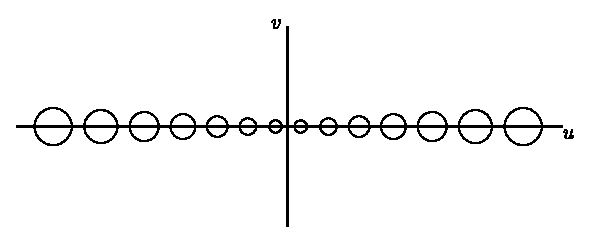
\includegraphics{figure/fig76-1.1_1.eps}
\caption{}
\end{figure}


This\pageoriginale explains why it is not possible to find an
exhaustive classification of the local zero sets of such mappings {\em
in geometrical terms}. Nevertheless, a partial classification if
possible. It will be obtained by the following. Given a mapping $f$
verifying $f(0) = 0, Df(0) = 0$, det $D^{2}f(0) = 0$ and $D^{2}f(0)
\neq 0$, we shall construct a new mapping $f^{(1)}$ whose local zero
set provides that of $f$ through an elementary transfomation. About the
mapping $f^{(1)}$, the following three possiblities are {\em
  exhaustive}:
\begin{enumerate}
\item[1)] $Df^{(1)} (0) \neq 0$ so that the local zero set of
  $f^{(1)}$ can be found through the Implicit function theorem.

\item[2)] $Df^{(1)} (0) = 0$, det $D^{2}f^{(1)} (0) \neq 0$ so that
  the local zero set of $f^{(1)}$ can be found through the Morse lemma.

\item[3)] $Df^{(1)} (0) = 0$, det $D^{2}f^{(1)}(0) = 0$ and
  $D^{2}f^{(1)} (0) \neq 0$ so that finding the local zero set of
  $f^{(1)}$ reduces to finding the local zero set of a new iterate $f^{(2)}$.
\end{enumerate}

In so doing, we define a sequence of iterates $f^{(1)}, \cdots,
f^{(m)}$: The iterate $f^{(m)}$ exists under the necessary and
sufficient condition that the local zero set of $f^{(m-1)}$ cannot be
found through the Implicit function theorem or the Morse lemma. If the
process ends after a finite number of steps, it corresponds to a {\em
  desingularization} of the initial mapping $f$. If it is endless, there
are two possibilities, among which one of them bears a geometric
characterization (see $\S\ 8$).

We shall complete this section by giving a definition and
establishing\pageoriginale a preliminary property. Of course, the
mapping $f$ will henceforth verify the condition $f(0) = 0$ and 
\begin{align*}
Df(0) & = 0,\tag{1.1}\label{chap5-eq1.1}\\
det D^{2}f(0) & = 0,\tag{1.2}\label{chap5-eq1.2}\\
D^{2}f(0) \neq 0.\tag{1.3}\label{chap5-eq1.3}
\end{align*}

In particular, (\ref{chap5-eq1.2}) means that the null-space of the
mapping $D^{2}f(0)\break \epsilon \mathscr{L}(\mathbb{R}^{2}, \mathscr{L}
(\mathbb{R}^{2}, \mathbb{R}))$ does not reduce to $\{0\}$. Because of
(\ref{chap5-eq1.3}), this null-space is not the whole space
$\mathbb{R}^{2}$ and it is then one-dimensional.

\begin{definition}\label{chap5-def1.1}
The one-dimensional space
$$
\Xi = \Ker D^{2}f(0),
$$
will be called the characteristic of $f$.
\end{definition}

The following elementary result will be used several times.

\begin{lemma}\label{chap5-lem1.1}
Under our assumptions, $D^{2}f(0) \cdot (\widetilde{\xi})^{2} = 0$ for
some $\widetilde{\xi} \epsilon \mathbb{R}^{2}$ if and only if
$\widetilde{\xi} \epsilon \Xi$.
\end{lemma}

\begin{proof}
It is obvious that $D^{2}f(0) \cdot (\widetilde{\xi})^{2} = 0$, if
$\widetilde{\xi} \epsilon \Xi$. Conversely, let $\widetilde{\xi}
\epsilon \mathbb{R}^{2}$ be such that $D^{2}f(0) \cdot
(\widetilde{\xi})^{2} = 0$ and assume by contradiction that there is
$\widetilde{\tau} \epsilon \mathbb{R}^{2}$ with $D^{2}f(0) \cdot
(\widetilde{\xi}, \widetilde{\tau}) \neq 0$. Necessarily,
$\widetilde{\xi}$ and $\widetilde{\tau}$ are not collinear, so that
$\{\widetilde{\xi}, \widetilde{\tau}\}$ is a basis of
$\mathbb{R}^{2}$. With respect to this basis, $D^{2}f(0)$ becomes
\begin{equation*}
\begin{bmatrix}
0 & D^{2}f(0) \cdot (\widetilde{\xi}, \widetilde{\tau})\\
D^{2}f(0) \cdot (\widetilde{\xi}, \widetilde{\tau}) & D^{2}f(0) \cdot (\widetilde{\tau})^{2}
\end{bmatrix}
\end{equation*}
and\pageoriginale its determinant is $- (D^{2}f(0) \cdot
(\widetilde{\xi}, \widetilde{\tau}))^{2} < 0$, which contradicts the
hypothesis that it vanishes\footnote{Recall that the condition det
  $D^{2}f(0) = 0$ is independent of the choice of any basis in $\mathbb{R}^{2}$.}.
\end{proof}

\section{Desingularization by Blowing-up Procedure.}\label{chap5-sec2}

We shall begin with an approach we have already used in Chapter
\ref{chap2}. Extending (in theory) the mapping $f$ to the whole space
$\mathbb{R}^{2}$ as a $C^{\infty}$ mapping, we first reduce the
problem of finding the non-zero solutions of the equation
$f(\widetilde{x}) = 0$ with prescribed euclidian norm
$||\widetilde{x}||$ to the problem
\begin{equation*}
\begin{cases}
& (t, \widetilde{x}) \epsilon (\mathbb{R} - \{0\}) \times S_{1},\\
& g(t, \widetilde{\xi}) = 0,
\end{cases}\tag{2.1}\label{chap5-eq2.1}
\end{equation*}
where the mapping $g$ defined on $\mathbb{R} \times \mathbb{R}^{2}$ with
values in $\mathbb{R}^{2}$ is given by
\begin{equation*}
g(t, \widetilde{\xi}) = 
\begin{cases}
\frac{1}{t^{2}} f(t\widetilde{\xi}) \text{ if } t \neq 0,\\
\frac{1}{2} D^{2}f(0) \cdot (\widetilde{\xi})^{2} \text{ if } t =
0.
\end{cases}\tag{2.2}\label{chap5-eq2.2} 
\end{equation*}

The relationship of the nonzero solutions $\widetilde{x}$ of the
equation $f(x) = 0$ to the solutions $(t, \widetilde{\xi})$ of the
equation $g(t, \widetilde{\xi}) = 0$ is of course that $\widetilde{x}$
can always be written as $\widetilde{x} = t\widetilde{\xi}$ (in two
different ways).

\begin{remark}\label{chap5-rem2.1}
The mapping $g$ in (\ref{chap5-eq2.2}) differs from that of Chapter
\ref{chap2} by the multiplicative factor $1/2$ only. This modification
will bring some\pageoriginale simplifications in the formulas later.
\end{remark}

Writing the Taylor expansion of $f$ about the origin, we find that 
\begin{equation*}
g(t, \widetilde{\xi}) = \int\limits_{0}^{1} (1-s)
D^{2}f(st\widetilde{\xi}) \cdot (\widetilde{\xi})^{2} ds,\tag{2.3}\label{chap5-eq2.3}
\end{equation*}
for every $(t, \widetilde{\xi}) \epsilon \mathbb{R} \times
\mathbb{R}^{2}$, which shows that the mapping $g$ is of class
$C^{\infty}$. The next result, very similar to Lemma
\ref{chap2-lem3.2} of Chapter \ref{chap2}, is based on the observation
that the intersection $S_{1} \cap \Xi$ reduces to two points. For the
sake of convenience, we shall say that two problems are {\em
  equivalent} if all the solutions of one of them provide all the
solutions of the other. We leave it to the reader to keep track of the
(obvious) correspondence between the solutions of the problems under
consideration.

\begin{lemma}\label{chap5-lem2.1}
Let $\widetilde{\xi}_{0}$ be either point of the intersection $\Xi
\cap S_{1}$ and C a given neighbourhood of $\widetilde{\xi}_{0}$ in
$S_{1}$. Then, for $r > 0$ small enough the problems
\begin{equation*}
\begin{cases}
& 0 < |t| < r, \widetilde{\xi} \epsilon S_{1},\\
& g(t, \widetilde{\xi}) = 0,
\end{cases}\tag{2.4}\label{chap5-eq2.4}
\end{equation*}
and 
\begin{equation*}
\begin{cases}
& 0 < |t| < r, \widetilde{\xi} \epsilon C,\\
& g(t, \widetilde{\xi}) = 0,
\end{cases}\tag{2.5}\label{chap5-eq2.5}
\end{equation*}
are equivalent.
\end{lemma}

\begin{proof}
First,\pageoriginale note that the problem (\ref{chap5-eq2.5}) is
equivalent to
\begin{equation*}
\begin{cases}
& 0 < |t| < r, \widetilde{\xi} \epsilon C \cup (-C)\\
& g(t, \widetilde{\xi}) = 0,
\end{cases}\tag{2.6}\label{chap5-eq2.6}
\end{equation*}
since each solution of (\ref{chap5-eq2.5}) is obviously a solution of
(\ref{chap5-eq2.6}) and conversely, given any solution $(t,
\widetilde{\xi})$ of (\ref{chap5-eq2.6}), either $(t,
\widetilde{\xi})$ or $(-t, -\widetilde{\xi})$ is a solution of
(\ref{chap5-eq2.5}) from the relation $g(t, \widetilde{\xi}) = g(-t,
-\widetilde{\xi})$. We shall prove the assertion by showing that the
problems (\ref{chap5-eq2.4}) and (\ref{chap5-eq2.6}) {\em have the
  same solutions} for $r > 0$ small enough. Each solution of
(\ref{chap5-eq2.6}) is clearly a solution of
(\ref{chap5-eq2.4}). Conversely, assume, by contradiction, that there
is no $r > 0$ such that each solution of (\ref{chap5-eq2.4}) is a
solution of (\ref{chap5-eq2.6}). This means that there is a sequence
$(t_{\ell}, \widetilde{\xi}_{\ell})_{\ell \geq 1}$ with $\lim\limits_{\ell
  \to + \infty} t_{\ell} = 0$, $\widetilde{\xi}_{\ell} \epsilon S_{1}
\ C \cup (-C)$ and $g(t_{\ell}, \widetilde{\xi}_{\ell}) = 0$. From the
compactness of $S_{1}$, we may assume that there is $\widetilde{\xi}
\epsilon S_{1}$ such that $\widetilde{\xi}_{\ell}$ converges to
$\widetilde{\xi}$. By the coninuity of $g$, we deduce $g(0,
\widetilde{\xi}) = 0$. But, by definition of $g(0, \cdot)$ and Lemma
\ref{chap5-lem1.1}, $\widetilde{\xi}$ must be one of the elements
$\widetilde{\xi}_{0}$ or $-\widetilde{\xi}_{0}$, which is impossible,
since $\widetilde{\xi}_{\ell} \notin C \cup (-C)$ for every $\ell \geq 1$,
by hypothesis.
\end{proof}

Let us now consider a subspace $T$ of $\mathbb{R}^{2}$ such that
\begin{equation*}
\mathbb{R}^{2} =- \Xi \oplus T.\tag{2.7}\label{chap5-eq2.7}
\end{equation*}

Given a non-zero element $\widetilde{\tau}_{0} \epsilon T$, we may
write $T = \mathbb{R}\widetilde{\tau}_{0}$. Let $\Phi : \mathbb{R}^{2}
\to \mathbb{R} \times S_{1}$ be the $C^{\infty}$ mapping defined by
\begin{equation*}
\Phi(u_{1}, v_{1}) = (u_{1} ||\widetilde{\xi}_{0} + v_{1}
\widetilde{\tau}_{0}||, (\widetilde{\xi}_{0} +
v_{1}\widetilde{\tau}_{0}) / ||\widetilde{\xi}_{0} + v_{1}\widetilde{\tau}_{0}||),\tag{2.8}\label{chap5-eq2.8}
\end{equation*}
(where\pageoriginale $|\cdot|$ still denotes the euclidean
norm). Clearly, $\Phi(0, 0) = (0, \widetilde{\xi}_{0})$ and an
elementary calculation yields
$$
D\Phi(0, 0) \cdot (u_{1}, v_{1}) = (u_{1}, v_{1} \widetilde{\tau}_{0}
- v_{1}(\widetilde{\xi}_{0} | \widetilde{\tau}_{0})\widetilde{\xi}_{0}),
$$
for $(u_{1}, v_{1}) \epsilon \mathbb{R}^{2}$, where $(\cdot | \cdot)$
denotes the inner product of $\mathbb{R}^{2}$. The above relation
shows that the mapping $D\Phi(0, 0)$ is one-to-one (as an element of
$\mathscr{L} (\mathbb{R}^{2}, \mathbb{R}^{3})$) and hence is an
isomorphism of $\mathbb{R}^{2}$ to $\mathbb{R} \times
T_{\widetilde{\xi}_{0}}S_{1} (= \mathbb{R} \times
\{\widetilde{\xi}_{0}\}^{\perp})$. Thus, $\Phi$ is a $C^{\infty}$
diffeomorphism between a neighbourhood of the origin in
$\mathbb{R}^{2}$ and a neighbourhood of the point $(0,
\widetilde{\xi}_{0})$ in $\mathbb{R} \times S_{1}$. We can suppose
that the latter contains the product $(-r, r) \times C$ of Lemma
\ref{chap5-lem2.1}: it suffices to choose $C$ small enough and shrink
$r > 0$ accordingly. Then, $\Phi^{-1} ((-r, r) \times C)$ is a
neighbourhood $W_{1}$ of the origin in $\mathbb{R}^{2}$ and each pair
$(t, \widetilde{\xi}) \epsilon (-r, r) \times$ has the form
\begin{equation*}
\begin{cases}
& t = u_{1} ||\widetilde{\xi}_{0} + v_{1}\widetilde{\tau}_{0}||,\\
& \widetilde{\xi} = (\widetilde{\xi}_{0} + v_{1}\widetilde{\tau}_{0})/
  ||\widetilde{\xi}_{0} + v_{1}\widetilde{\tau}_{0}||,
\end{cases}
\end{equation*}
with $(u_{1}, v_{1}) \epsilon W_{1}$. As $t = 0$ {\em if and only if}
$u_{1} = 0$ and from lemma \ref{chap5-lem2.1}. our initial problem
of finding the nonzero solutions $\widetilde{x}$ in the local zero set
of $f$ is equivalent to
\begin{equation*}
\begin{cases}
& (u_{1}, v_{1}) \epsilon W_{1}, u_{1} \neq 0,\\
& g(u_{1}||\widetilde{\xi}_{0} + v_{1}\widetilde{\tau}_{0}||,
  (\widetilde{\xi}_{0} + v_{1}\widetilde{\tau}_{0}) /
  ||\widetilde{\xi}_{0} + v_{1}\widetilde{\tau}_{0}||) = 0
\end{cases}
\end{equation*}

Coming\pageoriginale back to the definition of $g$
((\ref{chap5-eq2.2})), this also reads
\begin{equation*}
\begin{cases}
& (u_{1}, v_{1}) \epsilon W_{1}, u_{1} \neq 0,\\
f(u_{1}(\widetilde{\xi}_{0} + v_{1}\widetilde{\tau}_{0})) = 0.
\end{cases}
\end{equation*}

Finally, multipying by $1/u_{1}^{2}$, the problem becomes
\begin{equation*}
\begin{cases}
& (u_{1}, v_{1}) \epsilon W_{1}, u_{1} \neq 0,\\
& g(u_{1}, \widetilde{\xi}_{0} + v_{1}\widetilde{\tau}_{0}) = 0.
\end{cases}
\end{equation*}

We shall denote by $f^{(1)}$ the $C^{\infty}$ real-valued function of
two variables
\begin{align*}
f^{(1)} : (u_{1}, v_{1}) \epsilon \mathbb{R}^{2} \to f^{(1)}(u_{1},
v_{1}) &= g(u_{1}, \widetilde{\xi}_{0} + v_{1}
\widetilde{\tau}_{0})\\ 
&= \begin{cases}
\frac{1}{u_{1}^{2}} f(u_{1}\widetilde{\xi}_{0} + u_{1} v_{1}
\widetilde{\tau}_{0}) \text{ if } u_{1} \neq 0,\\
\frac{1}{2} v_{1}^{2} D^{2}f(0) \cdot (\widetilde{\xi}_{0})^{2} \text{
if } u_{1} = 0.
\end{cases}\tag{2.9}\label{chap5-eq2.9}
\end{align*}

From the above comments, the nonzero solutions $\widetilde{x}$ of the
equation $f(\widetilde{x})$ with $||x|| < r$ are of the form
\begin{equation*}
\widetilde{x} = u_{1}\widetilde{\xi}_{0} + u_{1}v_{1}\widetilde{\tau}_{0}\tag{2.10}\label{chap5-eq2.10}
\end{equation*}
with $(u_{1}, v_{1}) \epsilon W_{1}, u_{1} \neq 0$ and $f^{(1)}
(u_{1}, v_{1}) = 0$. Obviously, the characterization
(\ref{chap5-eq2.10}) remains true with the solution $\widetilde{x} =
0$ since $f^{(1)} (0, 0) = 0$. In other words, since the neighbourhood
$W_{1} = \Phi^{-1} ((-r, r) \times C)$ can be taken arbitrarily small
(by shrinking C and $r > 0$), {\em the problem reduces to finding the
  local zero set of} $f^{(1)}$, from which the local zero set of is
deduced through the transformation (\ref{chap5-eq2.10}).

\begin{remark}\label{chap5-rem2.2}
The\pageoriginale reader may wonder why we have not defined the mapping
$f^{(1)}$ by formula (\ref{chap5-eq2.9}) directly. Indeed, it is clear
that every element of the form (\ref{chap5-eq2.10}) with $(u_{1},
v_{1})$ in the local zero set of $f^{(1)}$ is in the local zero set of
$f$. But the problem is to show that {\em every} element in the local
zero set of $f$ is of the form (\ref{chap5-eq2.10}) with $(u_{1},
v_{1})$ in the local zero set of $f^{(1)}$, a fact that uses the
compactness of the unit circle $S_{1}$, essential in Lemma \ref{chap5-lem2.1}.
\end{remark}

\begin{comment}\label{chap5-com2.1}
The vector $\widetilde{\xi}_{0} \epsilon \Xi$ has been chosen so that
$\widetilde{\xi}_{0} \epsilon S_{1}$ i.e. $||\widetilde{\xi}_{0}|| =
1$. This is without importance and $\widetilde{\xi}_{0}$ can be taken
as an arbitrary non-zero element of the characteristic $\Xi$ (bu
changing the inner product of $\mathbb{R}^{2}$ for instance). From
now on, we shall allow this more general choice in the definition of
the mapping $f^{(1)}$ in (\ref{chap5-eq2.9}).
\end{comment}

All the derivatives of the mapping $f^{(1)}$ can be explicitly
computed in terms of the derivatives of $f$ at the origin. First from
(\ref{chap5-eq2.9}), for every pair $(j, \ell) \epsilon \mathbb{N}
\times \mathbb{N}$
$$
(\partial^{j+\ell} f^{(1)} / \partial u_{1}^{j}\partial
v_{1}^{\ell})(0) = (\partial^{j+\ell} g/\partial t^{j}\partial
\widetilde{\xi}^{\ell}) (0, \widetilde{\xi}_{0}) \cdot (\widetilde{\tau}_{0})^{\ell}.
$$

Now
\begin{lemma}\label{chap5-lem2.2}
For every pair $(j, \ell) \epsilon \mathbb{N} \times \mathbb{N}$, one
has
\begin{equation*}
(\partial^{j+\ell}  fg / \partial t^{j}\partial \widetilde{\xi}^{\ell})
  (0, \widetilde{\xi}) = 
\begin{cases}
& 0 \text{ if } \ell > j+2\\
& [j! / (j + 2 - \ell)!] D^{j+2} f(0) \cdot
  (\widetilde{\xi})^{j+2-\ell}\\
&\qquad\qquad \text{ if } 0 \leq \ell \leq j + 2,
\end{cases}\tag{2.11}\label{chap5-eq2.11}
\end{equation*}
for every $\widetilde{\xi} \epsilon \mathbb{R}^{2}$.
\end{lemma}

\begin{proof}
Using\pageoriginale the expression (\ref{chap5-eq2.3}) of $g$ and for
every pair $(t, \widetilde{\xi}) \epsilon \mathbb{R} \times
\mathbb{R}^{2}$, we find
$$
(\partial^{j} g / \partial t^{j}) (t, \widetilde{\xi}) =
\int\limits_{0}^{1} (1-s)s^{j}D^{j+2}f(st \widetilde{\xi}) \cdot
(\widetilde{\xi})^{j+2} ds.
$$

In particular, for $t = 0$,
$$
(\partial^{j} g/\partial t^{j})(0, \widetilde{\xi}) =
\frac{-1}{(j+1)(j+2)} D^{j+2} f(0) \cdot (\widetilde{\xi})^{j+2},
$$
and (\ref{chap5-eq2.11}) follows.
\end{proof}

With Lemma \ref{chap5-lem2.2}, we obtain for every pair $(j, \ell)
\epsilon \mathbb{N} \times \mathbb{N}$,
\begin{equation*}
(\partial^{j+\ell} f^{(1)} / \partial u_{1}^{j} \partial v_{1}^{\ell})
  (0) = 
\begin{cases}
& 0 \text{ if } \ell > j+2,\\
& [j!/(j+2-\ell)!] D^{j+2} f(0) \cdot
  ((\widetilde{\xi}_{0})^{j+2-\ell},\\ 
&\qquad\qquad (\widetilde{\tau}_{0})^{\ell})
  \text{ if } 0 \leq \ell < j+2.
\end{cases}\tag{2.12}\label{chap5-eq2.12}
\end{equation*}

In particular, taking $j = 0$ and $\ell = 2$ in formula
(\ref{chap5-eq2.12}), 
\begin{equation*}
(\partial^{2}f^{(1)} / \partial v_{1}^{2})(0) = D^{2}f(0) \cdot
  (\widetilde{\tau}_{0})^{2} \neq 0,\tag{2.13}\label{chap5-eq2.13}
\end{equation*}
since $\widetilde{\tau}_{0} \notin \Xi$ (cf. Lemma
\ref{chap5-lem1.1}).

\section[Solution Through the Implict Function....]{Solution Through the Implict Function Theorem : CUSP
  Bifurcation}\label{chap5-sec3}

Applying fromula (\ref{chap5-eq2.12}) with $j = 1, \ell = 0$ and $j =
0, \ell = 1$ successively, we get
\begin{equation*}
(\partial f^{(1)}/ \partial u_{1})(0) = \frac{1}{6} D^{3}f(0)\cdot (\widetilde{\xi}_{0})^{3}\tag{3.1}\label{chap5-eq3.1}
\end{equation*}
and 
$$
(\partial f^{(1)}/ \partial v_{1})(0) = \frac{1}{2} D^{2}f(0) \cdot
(\widetilde{\xi}_{0}, \widetilde{\tau}_{0}).
$$

But,\pageoriginale as $\widetilde{\xi}_{0} \epsilon \Xi$, $D^{2}f(0)
\bullet \widetilde{\xi}_{0} = 0$. Hence
\begin{equation*}
(\partial f^{(1)} / \partial v_{1})(0) = 0.\tag{3.2}\label{chap5-eq3.2}
\end{equation*}

From (\ref{chap5-eq3.1})-(\ref{chap5-eq3.2}), the Implict function
theorem can be used for finding the local zero set of $f^{(1)}$ if and
only if 
\begin{equation*}
D^{3}f(0) \cdot (\widetilde{\xi}_{0})^{3} \neq 0,\tag{3.3}\label{chap5-eq3.3}
\end{equation*}
a condition which is independent of the nonzero element
$\widetilde{\xi}_{0} \epsilon \Xi$ and of the space $T$ chosen for
defining the mapping $f^{(1)}$. Assume then that (\ref{chap5-eq3.3})
holds. The Implict function theorem states that the local zero set of
$f^{(1)}$ is made of exactly one curve of class $C^{\infty}$. Due to
(\ref{chap5-eq3.2}), this curve is tangent to the $v_{1}$-axis at the
origin. In other words, around the origin
$$
f^{(1)}(u_{1}, v_{1}) = 0 \Leftrightarrow u_{1} = u_{1}(v_{1}),
u_{1}(0) = (du_{1}/dv_{1})(0) = 0.
$$

This result can be made more precise by showing that $(d^{2}u_{1} /
dv_{1}^{2})\break (0) \neq 0$: Differentiating two times the identity
$f^{(1)} (u_{1}(v_{1}), v_{1}) = 0$ and since $(du_{1} / dv_{1}) (0) =
(\partial f^{(1)} / \partial v_{1})(0) = 0$, we obtain
\begin{equation*}
(d^{2}u_{1}/dv_{1}^{2})(0) = - \frac{(\partial^{2}f^{(1)}/ \partial
    v_{1}^{2})(0)}{(\partial f^{(1)} / \partial u_{1})(0)} = -
  6\frac{D^{2}f(0) \cdot (\widetilde{\tau}_{0})^{2}}{D^{3}f(0) \cdot
    (\widetilde{\xi}_{0})^{3}} \neq 0,\tag{3.4}\label{chap5-eq3.4}
\end{equation*}
as it follows from (\ref{chap5-eq2.13}). In the $(u_{1},
v_{1})$-plane, the graph of the function $u_{1}(\cdot)$ is then as in
Figure 3.1

\setcounter{figure}{0}
\begin{figure}[H]
\centering
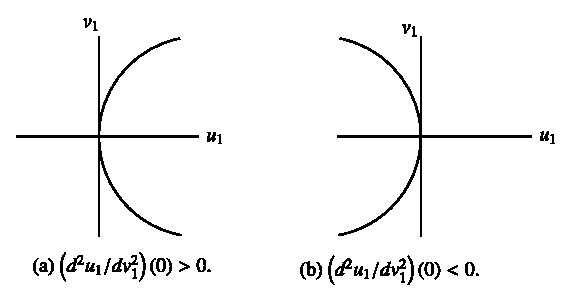
\includegraphics{figure/fig76-3.1_2.eps}
\caption{Local zero set of $f^{(1)}$}
\end{figure}


After\pageoriginale changing the vector $\widetilde{\xi}_{0}$ into
$-\widetilde{\xi}_{0}$ if necessary, we may assume
(cf. (\ref{chap5-eq3.4}))
\begin{equation*}
(d^{2}u_{1} / dv_{1}^{2})(0) > 0.\tag{3.5}\label{chap5-eq3.5}
\end{equation*}

\begin{theorem}\label{chap5-thm3.1}
The vector $\widetilde{\xi}_{0}$ being chosen so that
(\ref{chap5-eq3.5}) holds, let us set $\Xi_{+} = \mathbb{R}_{+}
\widetilde{\xi}_{0}$. Then, the local zero set of $f$ is made up of two
continuous half-branches emerging from the origin in the half space
$\Xi_{+} \oplus T$. These half-branches are of class $C^{\infty}$ away
from the origin and tangent to the characteristic $\Xi = \mathbb{R}
\widetilde{\xi}_{0}$ at the origin. More precisely, there exists an
origin-preserving $C^{\infty}$ diffeomorphism $\psi$ in $\mathbb{R}$
such that the local zero set of $f$ is made up of the two
half-branches\pageoriginale ($\rho > 0$ small enough)
\end{theorem}

\begin{proof}
After changing the vector $\widetilde{\tau}_{0}$ into a scalar
multiple, we may assume that $(d^{2}u_{1} / dv_{1}^{2})(0) = 2$
(cf. (\ref{chap5-eq3.4})). Not changing $\widetilde{\tau}_{0}$
introduces positive multiplicative constants in the expressions below
without (of course) affecting the final result. Thus
\begin{equation*}
u_{1}(v_{1}) = v_{1}^{2}(1 + R(v_{1})),\tag{3.7}\label{chap5-eq3.7}
\end{equation*}
where $R$ is a $C^{\infty}$ function such that $R(0) = 0$. The mapping 
\begin{equation*}
\varphi(v_{1}) = v_{1}(1 + R(v_{1}))^{1/2},\tag{3.8}\label{chap5-eq3.8}
\end{equation*}
is well defined and of class $C^{\infty}$ around the origin. In
addition
\begin{align*}
\varphi(0) & = 0,\\
\frac{d\varphi}{dv_{1}}(0) & = 1.
\end{align*}

It follows that $\varphi$ is an origin-preserving $C^{\infty}$ local
diffeomorphism of $\mathbb{R}$ and the relation (\ref{chap5-eq3.7}) is
simply
$$
u_{1}(v_{1}) = (\varphi(v_{1}))^{2}.
$$

From our choice of $\varphi$(\ref{chap5-eq3.8}), we see that
\begin{align*}
\varphi(v_{1}) & = \sqrt{u_{1} (v_{1})} \text{ if } v_{1} > 0,\\
\varphi(v_{1}) & = -\sqrt{u_{1} (v_{1})} \text{ if } v_{1} < 0.
\end{align*}

Setting $\psi = \varphi^{-1}$, we find
\begin{align*}
v_{1} & = \psi (\sqrt{u_{1}(v_{1})}) \text{ if } v_{1} \geq 0.\\
v_{1} & = \psi(- \sqrt{u_{1} (v_{1})}) \text{ if } v_{1} \leq 0.
\end{align*}\pageoriginale
\end{proof}

As $u_{1}(v_{1})$ runs over some interval $[0, \rho)$ for $v_{1}$
  around the origin. It is equivalent to saying, for every $u_{1}
  \epsilon [0, \rho[,$ that the two values $v_{1}$ with $u_{1} =
      u_{1}(v_{1})$ are given by $v_{1} = \pm \psi (\sqrt{u_{1}})$.

According toi the general discussion before, the local zero set of $f$
is made up of elements of the form
$$
\widetilde{x} = u_{1}\widetilde{\xi}_{0} + u_{1}v_{1}\widetilde{\tau}_{0},
$$
with $(u_{1}, v_{1})$ in the local zero set of $f^{(1)}$. Here, we
have then 
$$ 
\widetilde{x} = \widetilde{x}^{(\alpha)}(u_{1}) =
u_{1}\widetilde{x}_{0} + u_{1}\psi((-1)^{\alpha}\sqrt{u_{1}})\widetilde{\tau}_{0}
$$
for $u_{1} \epsilon [0, r)$. Dividing by $u_{1} \neq 0$, we get
$$ 
\lim_{u_{1} \to 0} \frac{\widetilde{x}^{(\alpha)}(u_{1})}{u_{1}} =
\widetilde{\xi}_{0} + \lim_{u_{1} \to 0} \psi((-1)^{\alpha}
\sqrt{u_{1}}) \widetilde{\tau}_{0} = \widetilde{\xi}_{0}
$$

This relation expresses that the two half-branches are tangent to the
characteristic $\Xi$ at the origin. They are distinct since
$\psi(\sqrt{u_{1}})$ and $\psi(-\sqrt{u_{1}})$ have opposite signs.

From Theorem \ref{chap5-thm3.1}, the local zero set of $f$ is then given
by Figure 3.2 below.
\begin{figure}[H]
\centering
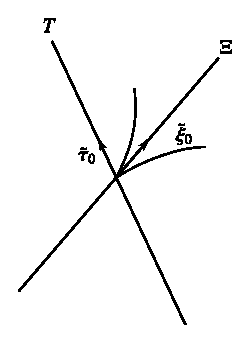
\includegraphics{figure/fig76-3.2_2.eps}
\caption{Local zero set of $f$.}
\end{figure}


Setting\pageoriginale $\widetilde{x} = (u, v)$, the simplest example
of mapping $f$ for which the hypothesis of this section are fulfilled is
$f(u, v) = u^{2} \pm v^{3}$ (or $v^{2} \pm u^{2}$, or, with $\theta$
any fixed real number, $(v \cos \theta - u \sin \theta)^{2} \pm (u
\cos \theta + v \sin \theta)^{3}$). This kind of bifurcation is
observed in chemical reaction problems (cf. Golubitsky and Keyfitz \cite{13}).


\section[Solution Through the Morse Lemma....]{Solution Through the Morse Lemma : Isolated Solution and
  Double Limit Bifurcation.}\label{chap5-sec4} 

As we saw in the previous section, a necessary and sufficient
condition for the local zero set of the mapping $f^{(1)}$
(\ref{chap5-eq2.9}) to be found through the Implicit function theorem
is $D^{3}f(0) \cdot (\widetilde{\xi}_{0})^{3} \neq 0$.\pageoriginale
Here, we shall then assume
\begin{equation*}
D^{3}f(0) \cdot (\widetilde{\xi}_{0})^{3} = 0.\tag{4.1}\label{chap5-eq4.1}
\end{equation*}

As a result, from (\ref{chap5-eq3.1}) and (\ref{chap5-eq3.2})
\begin{equation*}
(\partial f^{(1)} / \partial u_{1})(0) = (\partial f^{(1)} / \partial
  v_{1})(0) = 0.\tag{4.2}\label{chap5-eq4.2}
\end{equation*}

Let us now examine the second derivative.Taking $j = 2 \ell = 0$ and
$j = 1, \ell = 1$ successively in (\ref{chap5-eq2.12}), we find
\begin{align*}
& (\partial^{2}f^{(1)} / \partial u_{1}^{2}) (0) = \frac{1}{12}
  D^{4}f(0) \cdot
  (\widetilde{\xi}_{0})^{4},\tag{4.3}\label{chap5-eq4.3}\\
& (\partial^{2}f^{(1)}/ \partial u_{1} \partial v_{1}) (0) =
  \frac{1}{2} D^{3}f(0) \cdot ((\widetilde{\xi}_{0})^{3},
  \widetilde{\tau}_{0})\tag{4.4}\label{chap5-eq4.4} 
\end{align*}
and we already know that (cf. (\ref{chap5-eq2.13}))
\begin{equation*}
(\partial^{2}f^{(1)} / \partial v_{1}^{2})(0) = D^{2}f(0) \cdot
  (\widetilde{\tau}_{0})^{2} \neq 0. \tag{4.5}\label{chap5-eq4.5}
\end{equation*}

Therefore, the structure of the local zero set of the mapping
$f^{(1)}$ can be found through the Morse lemma if and only if the
determinant det $D^{2}f^{(1)}(0)$ is $\neq 0$. From the above, this
becomes
{\fontsize{10}{12}\selectfont
\begin{equation*}
det D^{2}f^{(1)}(0) = \frac{1}{12} (D^{4} f(0) \cdot
(\widetilde{\xi}_{0})^{4}) (D^{2}f(0) \cdot
(\widetilde{\tau}_{0})^{2}) - \frac{1}{4} (D^{3}f(0) \cdot
(\widetilde{\xi}_{0})^{2}, \widetilde{\tau}_{0})^{2} \neq 0. \tag{4.6}\label{chap5-eq4.6}
\end{equation*}}

Clearly, det $D^{2}f^{(1)} (0)$ being non-zero or not is independent
of the choice of the non-zero elements $\widetilde{\xi}_{0} \epsilon
\Xi$ and $\widetilde{\tau}_{0} \epsilon T$. It is true, but not as
obvious, that our assumptions are independent of the complement $T$ of
the characteristic $\Xi$ chosen for defining the mapping $f^{(1)}$. We
prove this in

\begin{proposition}\label{chap5-prop4.1}
The condition: $Df^{(1)} (0) = 0$ and det $D^{2}f^{(1)} (0) \neq 0$
is independent of the choice of the complement $T$ of the characteristic $\Xi$.
\end{proposition}

\begin{proof}
We\pageoriginale already know that the condition $Df^{(1)} (0) = 0$
(i.e. (\ref{chap5-eq4.1})) is independent of $T$. {\em Assuming}
$Df^{(1)}(0) = 0$, we shall see that the condition det
$D^{2}f^{(1)}(0) \neq 0$ is independent of $T$ too (see Remark
\ref{chap5-rem4.1} below). This can be checked directly on the formula
(\ref{chap5-eq4.6}) but we prefer here to give the {\em reason} why
this independence is true. The second derivative $D^{2}f(0,
\widetilde{\xi})$ of the mapping $g$ ((\ref{chap5-eq2.2})) is an element
of $\mathscr{L}(\mathbb{R} \times \mathbb{R}^{2},
\mathscr{L}(\mathbb{R} \times \mathbb{R}^{2}, \mathbb{R}))$ and our
assertion will follow from the equivalence
$$
det D^{2}f^{(1)}(0) \neq 0 \Leftrightarrow \Ker D^{2}g(0,
\widetilde{\xi}_{0}) = \{0\} \times \Xi,
$$
since $\Ker D^{2}g(0, \widetilde{\xi}_{0})$ is of course independent of
any choice of $T$.
\end{proof}

Let then $(t, \widetilde{\xi}) \epsilon \mathbb{R} \times
\mathbb{R}^{2}$ be in the null-space $\Ker D^{2}g(0,
\widetilde{\xi}_{0})$. This means
\begin{equation*}
\begin{cases}
& t(\partial^{2} g / \partial t^{2})(0, \widetilde{\xi}_{0}) +
  (\partial^{2}g/\partial t \partial \widetilde{\xi})(0,
  \widetilde{\xi}) \cdot \widetilde{\xi} =  0 \epsilon \mathbb{R},\\
& t(\partial^{2}g / \partial t \partial \widetilde{\xi})(0,
  \widetilde{\xi}_{0}) + (\partial^{2}g/\partial
  \widetilde{\xi}^{2})(0, \widetilde{\xi}_{0}) \cdot \widetilde{\xi} =
  0 \epsilon \mathscr{L}(\mathbb{R}^{2}, \mathbb{R})
\end{cases}\tag{4.7}\label{chap5-eq4.7}
\end{equation*}

From Lemma \ref{chap5-lem2.2},
\begin{align*}
& (\partial^{2} g/ \partial t^{2})(0, \widetilde{\xi}_{0}) =
  \frac{1}{12} D^{4}f(0) \cdot (\widetilde{\xi}_{0})^{4} \epsilon
  \mathbb{R},\tag{4.8}\label{chap5-eq4.8}\\
& (\partial^{2}g/\partial t \partial \widetilde{\xi})(0,
  \widetilde{\xi}_{0}) = \frac{1}{2} D^{3}f(0) \cdot
  (\widetilde{\xi}_{0})^{2} \epsilon \mathscr{L}(\mathbb{R}^{2},
  \mathbb{R}),\tag{4.9}\label{chap5-eq4.9}\\
& (\partial^{2}g/\partial \widetilde{\xi}^{2})(0, \widetilde{\xi}_{0})
  = D^{2}f(0) \epsilon \mathscr{L}(\mathbb{R}^{2},
  \mathscr{L}(\mathbb{R}^{2}, \mathbb{R})).\tag{4.10}\label{chap5-eq4.10}
\end{align*}

Since $\widetilde{\xi}_{0} \epsilon \Xi$, one has $D^{2}f(0) \cdot
\widetilde{\xi}_{0} = 0 \epsilon \mathscr{L}(\mathbb{R}^{2},
\mathbb{R})$. From (\ref{chap5-eq4.1}) and the above relations, the
equations (\ref{chap5-eq4.7}) are satisfied with $t = 0$ and
$\widetilde{\xi} = \widetilde{\xi}_{0}$, which shows that the line
$\{0\} \times \Xi$ is in the null-space Ker\pageoriginale $D^{2}g(0,
\widetilde{\xi}_{0})$. To prove that thie line is the whole null-space
and because the system $\{\widetilde{\xi}_{0}, \widetilde{\tau}_{0}\}$
is a basis of $\mathbb{R}^{2}$, it suffices to show with
$\widetilde{\xi} = \lambda\widetilde{\tau}_{0}, \lambda \epsilon
\mathbb{R}$, that the equations (\ref{chap5-eq4.7}) have no solution
other than $t = \lambda = 0$. With
(\ref{chap5-eq4.8})-(\ref{chap5-eq4.10}), they become
\begin{equation*}
\begin{cases}
& \frac{t}{12} D^{4}f(0) \cdot (\widetilde{\xi}_{0})^{4} +
\frac{\lambda}{2} D^{3}f(0) \cdot ((\widetilde{\xi}_{0})^{2},
\widetilde{\tau}_{0}) = 0 \epsilon \mathbb{R},\\
& \frac{t}{2} D^{3}f(0) \cdot (\widetilde{\xi}_{0})^{2} + \lambda
D^{2}f(0) \cdot \widetilde{\tau}_{0} = 0 \epsilon
\mathscr{L}(\mathbb{R}^{2}, \mathbb{R}).
\end{cases}\tag{4.11}\label{chap5-eq4.11}
\end{equation*}

The second equation (\ref{chap5-eq4.11}) is equivalent to two scalar
equations, obtained, for instance, by expressing that the value of the
left hand side vanishes at each of the two noncollinear vectors
$\widetilde{\xi}_{0}$ and $\widetilde{\tau}_{0}$. By the same
arguments as above (i.e. (\ref{chap5-eq4.1}) and $\widetilde{\xi}_{0}
\epsilon \Xi$)the first scalar equation is the trivial one $0 =
0$. The second equation is
\begin{equation*}
\frac{t}{2}D^{3}f(0) \cdot ((\widetilde{\xi}_{0})^{2},
\widetilde{\tau}_{0}) + \lambda D^{2}f(0) \cdot
(\widetilde{\tau}_{0})^{2} = 0.\tag{4.12}\label{chap5-eq4.12}
\end{equation*}

But the system made of (\ref{chap5-eq4.12}) and the first equation
(\ref{chap5-eq4.11}) has the unique solution $t = \lambda = 0$ if and
only if det $D^{2}f^{(1)} (0) \neq 0$ (cf. (\ref{chap5-eq4.6})), which
completes the proof.

\begin{remark}\label{chap5-rem4.1}
If $Df^{(1)} (0) \neq 0$ (i.e. $D^{3}f(0) \cdot
(\widetilde{\xi}_{0})^{3} \neq 0$), it is {\em not true} that the
condition det $D^{2}f^{(1)}(0) \neq 0$ is independent of the choice of
$T$, as the reader can easily check on formula (\ref{chap5-eq4.6}).
\end{remark}

\begin{remark}\label{chap5-rem4.2}
We could already make Proposition \ref{chap5-prop4.1} more precise by
showing that the {\em sign} of det $D^{2}f^{(1)}(0)$ is independent of
the choice of\pageoriginale $T$ (when $Df^{(1)} (0) = 0$) but this will
be an immediate consequence of our further analysis.
\end{remark}

\begin{theorem}\label{chap5-thm4.1}
Assume that $Df^{(1)} (0) = 0$.
\begin{enumerate}
\item[(i)] If det $D^{2}f^{(1)} (0) > 0$, i.e.
$$
\frac{1}{3} (D^{4}f(0) \cdot (\widetilde{\xi}_{0})^{4})(D^{2}f(0)
\cdot (\widetilde{\tau}_{0})^{2}) - (D^{3}f(0) \cdot
((\widetilde{\xi}_{0})^{2}, \widetilde{\tau}_{0}))^{2} > 0,
$$
the local zero set of $f$ reduces to the origin. 

\item[(ii)] If det $D^{2}f^{(1)}(0) < 0$, i.e. 
$$
\frac{1}{3} (D^{4}f(0) \cdot (\widetilde{\xi}_{0})^{4})(D^{2}f(0)
\cdot (\widetilde{\tau}_{0})^{2}) - (D^{3}f(0) \cdot
((\widetilde{\xi}_{0})^{2}, \widetilde{\tau}_{0}))^{2} < 0,
$$
the local zero set of $f$ consists of exactly two distinct curves of
class $C^{\infty}$, tangent to the characteristic $\Xi$ at the
origin. More precisely, there exist two real-valued functions
$v_{1}^{(\alpha)} (u_{1}), \alpha = 1, 2$, defined and of class
$C^{\infty}$ around the origin, verifying
\begin{equation*}
\frac{dv_{1}^{(1)}}{du_{1}} (0) \neq \frac{dv_{1}^{(2)}}{du_{1}}
(0),\tag{4.13}\label{chap5-eq4.13} 
\end{equation*}
such that the local zero set of f is made up of the two curves ($\rho
> 0$ small enough)
$$
u_{1} \epsilon (-\rho, \rho) \to \widetilde{x}^{(\alpha)}(u_{1}) =
u_{1}\widetilde{\xi}_{0} + u_{1}v_{1}^{(\alpha)}(u_{1})
\widetilde{\tau}_{0}, \alpha = 1, 2.
$$
\end{enumerate}
\end{theorem}

\begin{proof}
Recall that the local zero set of f is of the form
$$
\widetilde{x} = u_{1}\widetilde{\xi}_{0} + u_{1}v_{1}\widetilde{\tau}_{0},
$$
with $(u_{1}, v_{1})$ in the local zero set of $f^{(1)}$. The part (i)
is then obvious since the local zero set of $f^{(1)}$ reduces to the
origin.

Let\pageoriginale us now prove (ii). The local zero set of $f^{(1)}$
is made up of two $C^{\infty}$ curves intersecting transversaly at the
origin where their tangents are the two distinct lines of solutions of
the equation
$$
D^{2}f^{(1)}(0) \cdot (u_{1}, v_{1})^{2} = 0.
$$

Note that the $v_{1}$-axis is never one of these tangents since
$D^{2}f(0) \cdot (\widetilde{\tau}_{0})^{2} \neq 0$. As a result, the
projection of either tangent onto the $u_{1}$-axis and along the
$v_{1}$-axis a linear isomorphism and it follow that the two
$C^{\infty}$ curves can be parameterized by $u_{1}$ (cf. Figure 4.1
below)
\setcounter{figure}{0}
\begin{figure}[H]
\centering
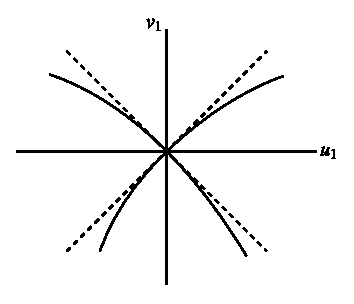
\includegraphics{figure/fig76-4.1.eps}
\caption{}
\end{figure}

More rigorously, each curve is of the form
\begin{equation*}
t \to (u_{1}(t), v_{1}(t)),\tag{4.14}\label{chap5-eq4.14}
\end{equation*}
a $C^{\infty}$ function around the origin verifying $u_{1}(0) =
v_{1}(0) = 0$ and 
$$
\frac{d}{dt} (u_{1}, v_{1}) |_{t=0} \neq 0
$$
(cf.Chapter \ref{chap2},  Corollary
\ref{chap2-coro3.1}).\pageoriginale Thus, the nonzero vector $((du_{1}/dt)(0)$,
$(dv_{1} / dt)(0))$ is tangent to the curve at the origin and, as it is
not collinear with the $v_{1}$-axis, one has
$$
\frac{du_{1}}{dt} (0) \neq 0.
$$

From the Inverse mapping theorem, the relation $u_{1} = u_{1}(t)$ is
equivalent to saying that $t = t(u_{1})$, a $C^{\infty}$ function
around the origin such that $t(0) = 0$. Therefore, the curve
(\ref{chap5-eq4.14}) is as well parametrized by
$$
u_{1} \to (u_{1}, v_{1}(t(u_{1})))
$$
as stated above. We have then proved that the local zero set of
$f^{(1)}$ is made of two $C^{\infty}$ curves $(u_{1}, v_{1}^{(\alpha)}
(u_{1})), \alpha = 1, 2$ and $u_{1} \epsilon (-\rho, \rho), \rho > 0$
small enough. As the vectors $(1, (dv_{1}^{(\alpha)} / du_{1})(0))$,
$\alpha = 1, 2$ are tangent to a different one of the two curves at
the origin (and hence are not collinear) we deduce
$$
\frac{dv_{1}^{(1)}}{du_{1}} (0) \neq \frac{dv_{1}^{(2)}}{du_{1}} (0).
$$

Finally, the local zero set of $f$ is made of the two $C^{\infty}$
curves
$$
u_{1} \epsilon (-\rho, \rho) \to \widetilde{x}^{(\alpha)}(u_{1}) =
u_{1}\widetilde{\xi}_{0} + u_{1}v_{1}^{(\alpha)} (u_{1})
\widetilde{\tau}_{0}, \alpha = 1, 2.
$$

Both are tangent to the characteristic $\Xi$ at the origin since
$$
\frac{d\widetilde{x}^{(\alpha)}}{du_{1}} (0) = \widetilde{\xi}_{0},
\alpha = 1, 2,
$$
and\pageoriginale they are distinct, since their second derivatives at
the origin
$$
\frac{d^{2} \widetilde{x}^{(\alpha)}}{du_{1}^{2}} (0) =
\frac{dv_{1}^{(\alpha)}}{du_{1}} (0), 
$$
differ.
\end{proof}

\begin{remark}\label{chap5-rem4.3}
We get an a posteriori proof of the fact that the sign of det
$D^{2}f^{(1)} (0)$ is independent of the choice of the space $T$ because
this sign is related to the {\em structure of the local zero set of $f$}.
\end{remark}

We shall noe describe a convenient way for finding the local zero set
of $f$ from that of $f^{(1)}$. It wil be repeatedly used in the
applications of the next section and we shall refer to it as the
``{\em quadrant method}''.

Identify the sum $\Xi \oplus T$ with the product
$\mathbb{R}\widetilde{\xi}_{0} \times \mathbb{R}
\widetilde{\tau}_{0}$, the vector $\widetilde{\tau}_{0}$ being chosen
so that ${\widetilde{\xi}_{0}, \widetilde{\tau}_{0}}$ is a direct
system of coordinates. In the $(u_{1}, v_{1})$-plane as well as in the
product $\mathbb{R} \widetilde{\xi}_{0} \times \mathbb{R}
\widetilde{\tau}_{0}$, we shall distinguish the usual four quadrants
(I), (II), (III) and (IV).
\begin{figure}[H]
\centering
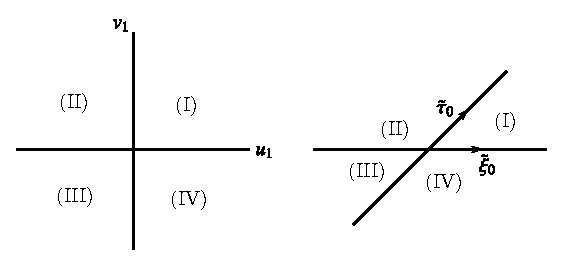
\includegraphics{figure/fig76-4.1_1.eps}
\end{figure}


Clearly,\pageoriginale the mapping
$$
(u_{1}, v_{1}) \to u_{1}\widetilde{\xi}_{0} + u_{1}v_{1}\widetilde{\tau}_{0},
$$
maps the quadrants $(I), \cdots , (IV)$ of the $(u_{1}, v_{1})$-plane
into the quadrants $(I), \cdots , (IV)$ of $\mathbb{R}
\widetilde{\xi}_{0} \times \mathbb{R} \widetilde{\tau}_{0}$ according
to the rule
\begin{align*}
& (I) \to (I) & (III) \to (II)\\
& (II) \to (III) & (IV) \to (IV)
\end{align*}

Thus, each half-branch in the local zero set of $f^{(1)}$ located in
(I) (resp. (II), (III), (IV)) is transformed into a half-branch in the
local zero set of $f$ located in (I) (resp. (III), (II), (IV)). Figure
4.2 below features some possible diagrams. The simplest example of a
mapping $f$ verifying the conditions of this section is $f(u, v) = u^{2}
\pm v^{4}$ (or $v^{2} \pm u^{4}$ or, with $\theta$ any fixed real
number, $(v \cos \theta - u \sin \theta)^{2} \pm (u \cos \theta + v
\sin \theta)^{4}$).
\begin{figure}[H]
\centering
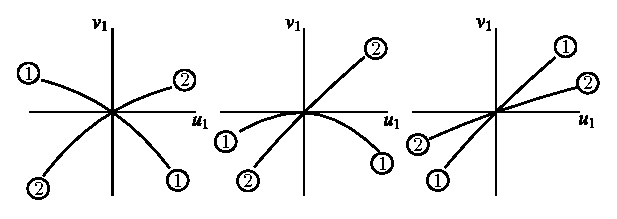
\includegraphics{figure/fig76-4.2a.eps}
\caption{(a) local zero set of $f^{(1)}$.}
\end{figure}

\setcounter{figure}{1}
\begin{figure}[H]
\centering
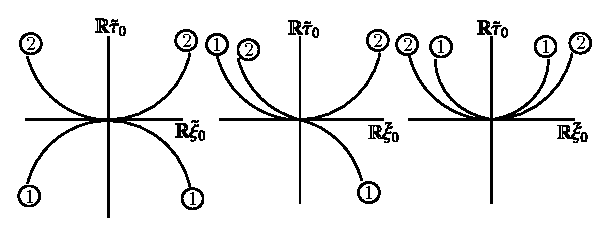
\includegraphics{figure/fig76-4.2b.eps}
\caption{(b) local zero set of $f$}
\end{figure}


\section{Iteration of the Process.}\label{chap5-sec5}

We\pageoriginale shall now assume that the local zero set of the
mapping $f^{(1)}$ cannot be determined through either the Implict
function theorem of the Morse lemma, that is to say
\begin{align*}
Df^{(1)} (0) & = 0,\tag{5.1}\label{chap5-eq5.1}\\
det D^{2}f^{(1)}(0) & = 0.\tag{5.2}\label{chap5-eq5.2} 
\end{align*}

From (\ref{chap5-eq2.13}), we know that $(\partial^{2}f^{(1)} /
\partial v_{1}^{2}) (0) \neq 0$. In particular,
\begin{equation*}
D^{2}f^{(1)}(0) \neq 0,\tag{5.3}\label{chap5-eq5.3}
\end{equation*}
and the problem of finding the local set of $f^{(1)}$ is the same as
considered in $\S 2$ with the mapping $f$. The mapping $f^{(1)}$ has a
characteristic\pageoriginale  $\Xi_{1}$ which is a one-dimensional subspace of the
$(u_{1}, v_{1})$-plane; considering any complement $T_{1}$ of
$\Xi_{1}$ and choosing arbitrary nonzero elements
$\widetilde{\xi}_{1}$ and $\widetilde{\tau}_{1}$ in $\Xi_{1}$ and
$T_{1}$ respectively,we can reduce the problem to finding the local
zero set of a new mapping $f^{(2)}$ obtained by blowing-up $f^{(1)}$
along $\Xi_{1}$. The mapping $f^{(2)}$ depends on the new variables
$(u_{2}, v_{2})$ through the relation
\begin{equation*}
f^{(2)} (u_{2}, v_{2}) = 
\begin{cases}
& \frac{1}{u_{2}^{2}} f^{(1)} (u_{2}\widetilde{\xi}_{1} + u_{2}v_{2}
\widetilde{\tau}_{1}) \text{ for } u_{2} \neq 0,\\
& \frac{1}{2} v_{2}^{2}D^{2} f^{(1)} (0) \cdot
(\widetilde{\tau}_{1})^{2} \text{ for } u_{2} = 0.
\end{cases}
\end{equation*}

An important observation is that the relation $(\partial^{2}f^{(1)} /
\partial v_{1}^{2})(0) \neq 0$ {\em keeps the characteristic $\Xi_{1}$ from
being the $v_{1}$-axis}. This will be summarized by saying that the
characteristic $\Xi_{1}$ is {\em not vertical}. Such a notion makes no
sense as far as the characteristic $\Xi$ is concerned, unless we {\em
  arbitrarily} fix a system $(u, v)$ of coordinates in the original
plane $\mathbb{R}^{2}$.

If $Df^{(2)} (0) \neq 0$, the local zero set of $f^{(2)}$ can be found
through the Implicit function theorem. From Theorem
\ref{chap5-thm3.1}, we deduce the local zero set of $f^{(1)}$ and,
finally, the local zero set of $f$. If $Df^{(2)} (0) = 0$ and det
$D^{2}f^{(2)} (0) = 0$, the mapping $f^{(2)}$ has a characteristic
$\Xi_{2}$ {\em which is not vertical} in its ambient space $(u_{2},
v_{2})$ and the problem reduces to finding the local zero set of a
third iterate $f^{(3)}$ depending on the new variables $(u_{3},
v_{3})$. More generally, we\pageoriginale have

\begin{theorem}\label{chap5-thm5.1}
Assume that the iterates $f^{(1)}, \cdots , f^{(m)}$ are defined and
$Df^{(m)} (0) \neq 0$. After changing $\widetilde{\xi}_{0}$ into
$-\widetilde{\xi}_{0}$ if necessary and setting $\Xi_{+} =
\mathbb{R}_{+} \Xi$, the local zero set of $f$ is made up of two
continuous half-branches emerging from the origin in the half-space
$\Xi_{+} \oplus T$. These half-branches are of class $C^{\infty}$ away
from the origin and tangent to the characteristic $\Xi$ at the origin.
\end{theorem}

\begin{proof}
The mappings $f^{(1)}, \cdots, f^{(m)}$ are defined after the choice
of non zero elements $\widetilde{\xi}_{0}, \cdots,
\widetilde{\xi}_{m-1}$ and $\widetilde{\tau}_{0}, \cdots ,
\widetilde{\tau}_{m-1}$ in the characteristics $\Xi,\break \Xi_{1}, \cdots
\Xi_{m-1}$ and some given complements $T, T_{1}, \cdots, T_{m-1}$. In
the $(u_{j},\break v_{j})$ plane, $\widetilde{\xi}_{j}$ and
$\widetilde{\tau}_{j}$ are of the form $\widetilde{\xi}_{j} =
(\alpha_{j}, \beta_{j})$ and $\widetilde{\tau}_{j} = (\lambda_{j},
\mu_{j})$, with $\alpha_{j} \neq 0$ {\em since the characteristic $\Xi_{j}$
is not vertical} for $1 \leq j \leq m-1$.
\end{proof}

Clearly, the iterate $f^{(m)}$ is the first iterate of
$f^{(m-1)}$. Thus, after changing $\widetilde{\xi}_{m-1}$ into
$-\widetilde{\xi}_{m-1}$, if necessary (which does not affect the
existence of the $m^{\rm th}$ iterate $f^{(m)}$ or the condition $Df^{(m)}(0)
\neq (0)$), we know from Theorem \ref{chap5-thm3.1} that the local
zero set of $f^{(m-1)}$ is made up of two half-branches ($\rho > 0$
small enough, $\psi$ an origin-presering $C^{\infty}$ local
diffeomorphism of $\mathbb{R}$)
$$
0 \leq u_{m} < \rho - \widetilde{x}_{m-1}^{(\alpha)} (u_{m}) =
u_{m}\widetilde{\xi}_{m-1} + u_{m}\psi((-1)^{\alpha} \surd
u_{m})\widetilde{\tau}_{m-1}, \alpha = 1, 2.
$$

In the system $(u_{m-1}, v_{m-1})$, this becomes
\begin{align*}
& u_{m-1}^{(\alpha)} (u_{m}) = \alpha_{m-1}u_{m} + \lambda_{m-1} u_{m}
\psi((-1)^{\alpha} \surd u_{m}),\\
& v_{m-1}^{(\alpha)} (u_{m}) = \beta_{m-1}u_{m} + \mu_{m-1} u_{m} \psi
((-1)^{\alpha} \surd u_{m}).\tag{5.4}\label{chap5-eq5.4}
\end{align*}

The\pageoriginale above mappings $u_{m-1}^{(\alpha)} (\cdot)$ and $v_{m-1}^{(\alpha)} (\cdot)$ are of class $C^{1}$ in $[0, \rho)$ with
\begin{equation*}
(du_{m-1}^{(\alpha)}/ du_{m}) (0) = \alpha_{m-1} \neq 0.\tag{5.5}\label{chap5-eq5.5}
\end{equation*}

Now, from $\S 2$, the local zero set of $f^{(m-2)}$ is made of elements of the form
$$
\widetilde{x}_{m-2} = u_{m-1} \widetilde{\xi}_{m-2} + u_{m-1} v_{m-1} \widetilde{\tau}_{m-2}, 
$$
with $(u_{m-1}, v_{m-1})$ in the local zero set of $f^{(m-1)}$. From (\ref{chap5-eq5.4}), $\widetilde{x}_{m-2} = \widetilde{x}_{m-2}^{(\alpha)} (u_{m}), \alpha = 1, 2$, with
$$
\widetilde{x}_{m-2} (u_{m}) = u_{m-1}^{(\alpha)} (u_{m})\widetilde{\xi}_{m-2} + u_{m-1}^{(\alpha)} (u_{m}) v_{m-1}^{(\alpha)} (u_{m}) \widetilde{\tau}_{m-2},
$$
which, in the system $(u_{m-2}, v_{m-2})$, expresses as
\begin{align*}
u_{m-2}^{(\alpha)} (u_{m}) & = \alpha_{m-2} u_{m-1}^{(\alpha)} (u_{m}) + \lambda_{m-2} u_{m-1}^{(\alpha)} (u_{m}) v_{m-1}^{(\alpha)} (u_{m}),\\
v_{m-2}^{(\alpha)} (u_{m}) & = \beta_{m-2} u_{m-1}^{(\alpha)} (u_{m}) + \mu_{m-2} u_{m-1}^{(\alpha)} (u_{m}) v_{m-1}^{(\alpha)} (u_{m}).
\end{align*}

The mappings $u_{m-2}^{(\alpha)} (\cdot) v_{m-2}^{(\alpha)} (\cdot)$ are of class $C^{1}$ in $(0, \rho)$ and, from (\ref{chap5-eq5.5})
$$
(du_{m-2}^{(\alpha)} . du_{m}) (0) = \alpha_{m-2} \alpha_{m-1} \neq 0, \alpha = 1, 2,
$$
since $\alpha_{m-2} \neq 0$. Iterating the process, we find that the local zero set of $f$ is of the form
$$
\widetilde{x}^{(\alpha)} (u_{m}) = u_{1}^{(\alpha)} (u_{m})\widetilde{\xi}_{0} + u_{1}^{(\alpha)} (u_{m}) v_{1}^{(\alpha)} (u_{m})\widetilde{\tau}_{0}, \alpha = 1, 2, 
$$
where the functions $u_{1}^{(\alpha)} (\cdot)$ and $v_{1}^{(\alpha)} (\cdot)$ are of class $C^{1}$ in $[0, \rho)$, vanish as the origin and
$$
(du_{1}^{(\alpha)} / du_{m})(0) = \alpha_{1} \cdots \alpha_{m-1} \neq 0.
$$

After\pageoriginale shrinking $\rho > 0$ if necessary, the sign of $u_{1}^{(\alpha)} (u_{m})$ is that of the product $\alpha_{1} \cdots \alpha_{m-1}$ for $0 < u_{m} < \rho$ and both values $\alpha = 1$ and $\alpha = 2$. Hence our assertion, since all the mappings we have considered are $C^{\infty}$ away from the origin.

When Theorem \ref{chap5-thm5.1} applies, the partical determination of the local zero set of $f$ from that of $f^{(m)}$ follows by successive applications of the ``quadrant method'' described in $\S 4$. Note, however, for $1 \leq j \leq m-1$, that the quadrants $(I), \cdots, (IV)$ used for finding the local zero set of $f^{(j)}$ from the local zero set of $f^{(j+1)}$ are (in general) {\em different} from the quadrants $(I), \cdots , (IV)$ used for finding the local zero set of $f^{(j-1)}$ from that of $f^{(j)}$.

Figure 5.1 (a), (b), (c) below gioves an example of the local zero set of $f^{(2)}, f^{(1)}$ and f respectively when Theorem \ref{chap5-thm5.1} applies with $m = 2$. A mapping whose local zero set looks like that in Figure 5.1(c) (and for which the process stops at $m = 2$ of course) is
$$
f(u, v) = (v-u^{2})^{2} + u^{5}.
$$
\setcounter{figure}{0}
\begin{figure}[H]
\centering
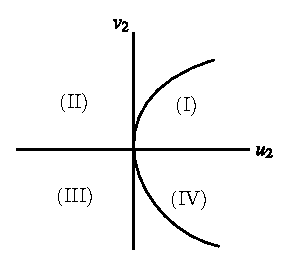
\includegraphics{figure/fig76-5.1a.eps}
\caption{(a) local zero set of $f^{(2)}$.}
\end{figure}

\setcounter{figure}{0}
\begin{figure}[H]
\centering
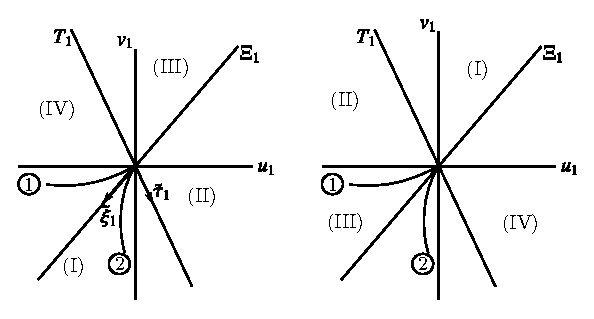
\includegraphics{figure/fig76-5.1b.eps}
\caption{(b) local zero set of $f^{(1)}$}
\end{figure}

\setcounter{figure}{0}
\begin{figure}[H]
\centering
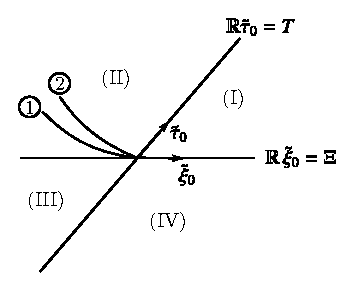
\includegraphics{figure/fig76-5.1c.eps}
\caption{(c) local zero set of $f$}
\end{figure}

\begin{remark}\label{chap5-rem5.1}
In\pageoriginale theory at least, applying Theorem \ref{chap5-thm5.1} does not require the computation of $f^{(1)}, \cdots, f^{(n)}$ and reduces to checking some conditions on the partial derivatives of $f$. For a general $m$, this follows from the proof of the {\em intrinsic character of the process}, namely,\pageoriginale that whether or not it stops at some rank $m$ with $Df^{(m)}(0) \neq 0$ is independent of the choice of the complements $T, T_{1}, \cdots, T_{m-1}$ and of the elements $\widetilde{\xi}_{0}, \cdots , \widetilde{\xi}_{m-1}$ and $\widetilde{\tau}_{0}, \cdots ,\widetilde{\tau}_{m-1}$ for defining the iterates $f^{(1)}, \cdots, f^{(m)}$\footnote{Observe that modifying $T, \cdots , T_{m-2}$ {\em affects} the characteristics $\Xi_{1}, \cdots , \Xi_{m-1}$ as well.}. For $m = 1$, this was shown in $\S\ 3$ (and the result is obvious). The proof of this assertion for any m is very technical and will not be given in these notes (cf. Rabier \cite{32})\footnote{However, $\S\ 6$ gives a partial result in this direction.}. We shall only give the example of the case when $m = 2$; The iterate $f^{(2)}$ is defined under the conditions (\ref{chap5-eq5.1}) and (\ref{chap5-eq5.2}), namely (cf. $\S\S 3$ and 4)
\begin{align*}
& D^{3}f(0) \cdot (\widetilde{\xi}_{0})^{3} = 0,\tag{5.6}\label{chap5-eq5.6}\\
& \frac{1}{3} (D^{4}f(0) \cdot (\widetilde{\xi})^{4}) (D^{2}f(0) \cdot (\widetilde{\tau}_{0})^{2}) - (D^{3}f(0) \cdot ((\widetilde{\xi}_{0})^{2}, \widetilde{\tau}_{0}))^{2} = 0.\tag{5.7}\label{chap5-eq5.7}  
\end{align*}

Now, a nonzero element $\widetilde{\xi}_{1}$ of the characterisitc $\Xi_{1}$ is
$$
\widetilde{\xi}_{1} = (D^{2}f(0) \cdot (\widetilde{\tau}_{0})^{2}), - \frac{1}{2} D^{3}f(0) \cdot ((\widetilde{\xi}_{0})^{2}, \widetilde{\tau}_{0})).
$$
From $\S 3$, the condition $Df^{(2)}(0) \neq 0$ is equivalent to
$$
D^{3}f^{(1)}(0) \cdot (\widetilde{\xi}_{1})^{3} \neq 0.
$$

Using (\ref{chap5-eq5.7}) and formula (\ref{chap5-eq2.12}), this can be rewritten as
\begin{align*}
\frac{4}{5} (D^{5}F(0) &\cdot(\widetilde{\xi}_{0})^{5}) (D^{2}f(0)
  \cdot (\widetilde{\tau}_{0})^{2}) - 8(D^{4}f(0)
  \cdot((\widetilde{\xi}_{0})^{3}, \widetilde{\tau}_{0}))(D^{3}f(0)\\ 
&\cdot ((\widetilde{\xi}_{0})^{2}, \widetilde{\tau}_{0})) + 4D^{3}f(0) \cdot (\widetilde{\xi}_{0}, (\widetilde{\tau}_{0})^{2})
(D^{4}f(0) \cdot (\widetilde{\xi}_{0})^{4}) \neq 0.\tag{5.8}\label{chap5-eq5.8}
\end{align*}
\end{remark}

When\pageoriginale (\ref{chap5-eq5.6}) and (\ref{chap5-eq5.7}) hold (which is independent of the choice of $\widetilde{\xi}_{0} \epsilon \Xi$ and $\widetilde{\tau}_{0}$ from Proposition \ref{chap5-prop4.1}), it is easy to see that (\ref{chap5-eq5.8}) also is independent of $\widetilde{\xi}_{0} \epsilon \Xi$ and $\widetilde{\tau}_{0}$. However, the reader can already guess that proving the intrinsic character of the process by using formulas such as (\ref{chap5-eq5.6})-(\ref{chap5-eq5.8}) is impossible in the general case.

Assume now that $Df^{(2)}(0) = 0$. Then, the local zero set of $f^{(2)}$ can be found through the Morse lemma and Theorem \ref{chap5-thm4.1} provides the structure of the local zero set of $f^{(1)}$, from which the structure of the local zero set of $f$ is easily derived. More generally, we have

\begin{theorem}\label{chap5-thm5.2}
Assume that the iterates $f^{(1)}, \cdots, f^{(m)}$ are defined and $Df^{(m)}(0) = 0$, det $D^{2}f^{(m)} (0) \neq 0$. Then, the local zero set of $f$ reduces to the origin if det $D^{2}f^{(m)}(0) > 0$ and is made up of exactly two distinct curves of class $C^{\infty}$ tangent to the characteristic $\Xi$ at the origin if det $D^{2}f^{(m)}(0) < 0$.
\end{theorem}

\begin{proof}
It is possible to parallel the proof of Theorem \ref{chap5-thm5.1}. However, we are going to give a more ``geometrical'' one. We limit ourselves to the case $m = 2$, the general situation being identical by repeating the same arguments. From $\S 2$ we know that the local zero set of $f$ is of the form
$$
\widetilde{x} = u_{1}\widetilde{\xi}_{0} + u_{1}v_{1}\widetilde{\tau}_{0},
$$
with $(u_{1}, v_{1})$ in the local zero set of $f^{(1)}$. The assertion is then obvious\pageoriginale if det $D^{2}f^{(2)}(0) > 0$ since the local zero set of $f^{(1)}$ reduces to the origin (cf. Theorem \ref{chap5-thm4.1}). Assume then that det $D^{2}f^{(2)}(0) < 0$ so that the local zero set of $f^{(1)}$ is made of two $C^{\infty}$ curves tangent to the characteristic $\Xi_{1}$ at the origin as Theorem \ref{chap5-thm4.1} states. In addition, from the proof of Theorem \ref{chap5-thm4.1}, these curves coincide with the graphs of two $C^{\infty}$ functions defined around the origin in $\Xi_{1}$ with values in $T_{1}$. The important point is that this property is not affected, if $T_{1}$ is replaced by any other complement of $T_{1}$ (express the general form of a linear change of coordinates leaving the characteristic $\Xi_{1}$ globally invariant and use the Implicit function theorem). In particular, as the characteristic $\Xi_{1}$ is not vertical, this complement can be taken as the $v_{1}$-axis $\mathbb{R}(0, 1)$. Thus, the local zero set of $f^{(1)}$ coincides with the graphs of two $C^{\infty}$ functions defined around the origin $\Xi_{1}$ with values in $\mathbb{R}(0, 1)$. Because the characterisitc $\Xi_{1}$ is not vertical again, its projection onto the $u_{1}$-axis is a linear isomorphism. It follows that the local zero set of $f^{(1)}$ coincides with the graphs of two $C^{\infty}$ functions $v_{1}^{(\alpha)} (u_{1}), \alpha = 1, 2,$ defined for $|u_{1}| < \rho(\rho > 0$ small enough) verifying $v_{1}^{(\alpha)} (0) = 0$. Hence, the local zero set of $f$ is made up of the two curves
$$
u_{1} \epsilon (-\rho, \rho) \to \widetilde{x}^{(\alpha)} (u_{1}) = u_{1}\widetilde{\xi}_{0} + u_{1}v_{1}^{(\alpha)} (u_{1})\widetilde{\tau}_{0}, \alpha = 1, 2.
$$

Theses two curves are tangent to the characteristic $\Xi$ at the origin and they are distinct, since they coincide with the graphs of the two distinct\pageoriginale functions $u_{1}v_{1}^{(\alpha)} (u_{1})$ in $\mathbb{R} \widetilde{\xi}_{0} \times \mathbb{R}\widetilde{\tau}_{0}$. Finally, they are of class $C^{\infty}$, since the functions $v_{1}^{(\alpha)}$ are and the proof is complete.
\end{proof}

For practically finding the local zero set of $f$ from the local zero set of $f^{(m)}$, the quadrant method can be applied again. We now show it on the example when
$$
f(u, v) = u^{2} + 2uv^{2} + u^{3} + 2u^{2} v + v^{4} + 2uv^{3} + uv^{4} + v^{5} + v^{6}.
$$

Clearly, $f(0) = 0, Df(0) = 0, D^{2}f(0) \neq 0$ and det $D^{2}f(0) = 0$. Here, the characteristic $\Xi$ is the space $\Xi = \mathbb{R} (0, 1)$. It is convenient to take $T = \mathbb{R}(1, 0)$ (however, the process being intrinsic, all the possible choices are equivalent). If so, with $\widetilde{\xi}_{0} = (0, 1)$ and $\widetilde{\tau}_{0} = (1, 0)$, we find
\begin{align*}
f^{(1)} (u_{1}, v_{1}) & = \frac{1}{u_{1}^{2}} f(u_{1}(0, 1) + u_{1}v_{1}(1, 0)) = \frac{1}{u_{1}^{2}} f(u_{1}v_{1}, u_{1}) = \\
& = v_{1}^{2} + 2u_{1}v_{1} + u_{1}v_{1}^{3} + u_{1}v_{1}^{2} + u_{1}^{2} + 2u_{1}^{2}v_{1} + u_{1}^{3}v_{1} + u_{1}^{3} + u_{1}^{4}.
\end{align*}

We see that $Df^{(1)}(0) = 0$ while the quadratic part of $f^{(1)}$ is $(u_{1} + v_{1})^{2}$. Thus, the characteristic $\Xi_{1}$ is $\Xi_{1} = \mathbb{R}(1, -1)$ and we choose $T_{1} = \mathbb{R}(0, 1)$. Taking $\widetilde{\xi}_{1} = (1, -1)$ and $\widetilde{\tau}_{1} = (0, 1)$, we find 
\begin{align*}
f^{(2)}(u_{2}, v_{2}) & = \frac{1}{u_{2}^{2}} f^{(1)}(u_{2}(1, -1) + u_{2}v_{2}(0, 1)) = \frac{1}{u_{2}^{2}} f^{(1)} (u_{2}, u_{2} (v_{2} - 1))\\
& = v_{2}^{2} - u_{2}^{2} + 4u_{2}^{2}v_{2} + u_{2}v_{2}^{2} + u_{2}^{2}v_{2}^{3} - 3u_{2}^{2}v_{2}^{2}.
\end{align*}

The mapping $f^{(2)}$ verifies $Df^{(2)}(0) = 0$ and det $D^{2}f^{(2)}(0) = -4 < 0$. The two lines in the local zero set of $D^{2}f^{(2)}(0) \cdot (u_{2}, v_{2})^{2}$ are the lines\pageoriginale $u_{2} = v_{2}$ and $u_{2} = -v_{2}$. Figure 5.2 showshow the quadrant method allows to find the two curves in the local zero set of $f$.
\begin{figure}[H]
\centering
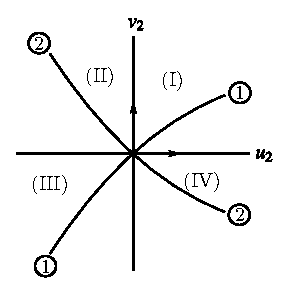
\includegraphics{figure/fig76-5.2a.eps}

{(a) local zero set of $f^{(2)}$}

\bigskip

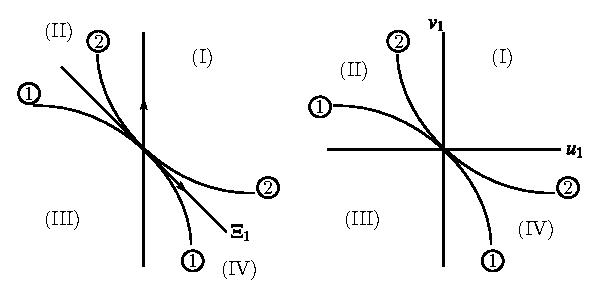
\includegraphics{figure/fig76-5.2b.eps}

{(b) local zero set of $f^{(1)}$}

\bigskip
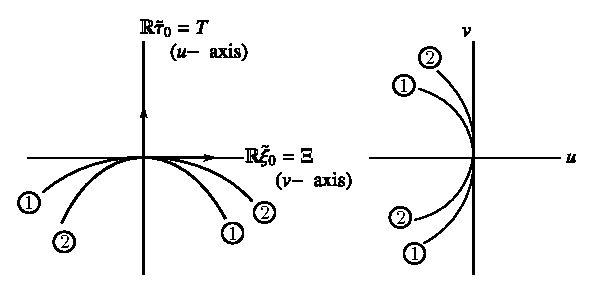
\includegraphics{figure/fig76-5.2c.eps}


{(c) local zero set of $f$}
\caption{}
\end{figure}


\section{Partial Results on the Intrinsic Character of the Process}\label{chap5-sec6}

A\pageoriginale natural question we have already mentioned is to know whether the process described in $\S 5$ is intrinsic or depends on the successive spaces $T, T_{1}, \cdots, T_{m-1}$ and elements $\widetilde{\xi}_{0}, \widetilde{\xi}_{1}, \cdots , \widetilde{\xi}_{m-1}$ and $\widetilde{\tau}_{0}, \widetilde{\tau}_{1}, \cdots, \widetilde{\tau}_{m-1}$ chosen for defining the iterates $f^{(1)}, \cdots, f^{(m)}$. In $\S\ 3$, we saw that the condition $Df^{(1)} (0) \neq 0$ was independent of the choice of $T$ and $\widetilde{\xi}_{0}, \widetilde{\tau}_{0}$ and we also proved a similar result as concerns the conditions $Df^{(1)}(0) = 0$ and det $D^{2}f^{(1)}(0) \neq 0$ {\em together} (cf. Proposition \ref{chap5-prop4.1}). The existence of a second iterate $f^{(2)}$ (i.e. the condition $Df^{(1)} (0) = 0$, det $D^{2}f^{(1)} (0) = 0$) is then independent of $T$ and $\widetilde{\xi}_{0}, \widetilde{\tau}_{0}$. Given such a space $T$ and elements $\widetilde{\xi}_{0} \epsilon \Xi, \widetilde{\tau}_{0} \epsilon T$ from which $f^{(1)}$ is defined, the existence of a third iterate $f^{(3)}$ is then independent of the choice of the complement $T_{1}$ of the characteristic $\Xi_{1}$ and of the non-zero elements $\widetilde{\xi}_{1} \epsilon \Xi_{1}$, $\widetilde{\tau}_{1} \epsilon T_{1}$. But whether or not its existence is independent of the initial choice  of $T$ and $\widetilde{\xi}_{0}, \widetilde{\tau}_{0}$ {\em is not ensured by our previous results}. However, we can reduce the question as follows. Since the characteristic $\Xi_{1}$ is not vertical and since the result is known to be independent of $T_{1}$, it suffices to prove that the existence of $f^{(3)}$ is independent of $T, \widetilde{\xi}_{0}, \widetilde{\tau}_{0}$ {\em when} $T_{1}$ {\em is taken as the} $v_{1}$-axis. Suppose then that this step has been solved successfully. We deduce that the existence of a fourth iterate $f^{(4)}$ is independent of the choice of $T_{1}, T_{2}$\pageoriginale and of the non-zero elements $\widetilde{\xi}_{1}, \widetilde{\xi}_{2}$ and $\tilde{\tau}_1, \tilde{\tau}_2$ in the characterisitcs $\Xi_{1}, \Xi_{2}$ and their complements $T_{1}, T_{2}$ respectively. Again, the non-dependence on the initial choice of $T$ and $\widetilde{\xi}_{0}, \widetilde{\tau}_{0}$ is not a consequence of the results we have established so far, but the problem can be reduced to the case when $T_{1}$ is taken as the $v_{1}$-axis and $T_{2}$ is taken as the $v_{2}$-axis. More generally, we see that proving that the process of $\S 5$ is intrinsic reduces to proving for every $m$ that it is independent of $T$ and  $\widetilde{\xi}_{0}, \widetilde{\tau}_{0}$ when the space $T_{1}, \cdots, T_{m-1}$ are taken as the $v_{1} -, \cdots, v_{m-1}$-axes.

Therefore, {\em we shall henceforth assume that the sequence $f^{(1)}, \ldots ,\break f^{(n)}$ is defined when $T_{j}$ is taken as the $v_{j}$-axis}, $1 \leq j \leq m-1$. Equivalently, we shall say that each space $T_{j}$, $1 \leq j \leq m-1$ is {\em vertical}. A proof of the independence of $T$ based on some generalization of Proposition \ref{chap5-eq4.1} is not available. Indeed, Proposition \ref{chap5-prop4.1} allows to prove the first independence result and is based on ``linear'' arguments while the question of the independence of $T$ in the general case is a {\em higher order (hence) nonlinear} problem. By showing that the two half-branches/curves (following that either Theorem \ref{chap5-thm5.1} or Theorem \ref{chap5-thm5.2} applies) in the local zero set of $f$ have a contact of order $m$ exactly at the origin, it is possible to establish that the process is intrinsic if, for choice of $T$, $Df^{(m)}(0) \neq 0$ or $Df^{(m)}(0) = 0$ and det $D^{2}f^{(m)} (0) < 0$ (thus, in such a case, $m$ and either condition $Df^{(m)}(0) \neq 0$ or $Df^{(m)} (0) = 0$ and det $D^{2}f^{(m)} (0) < 0$ is independent of $T$). If $Df^{(m)}(0) = 0$ and det $D^{2}f^{(m)} (0) > 0$, the local zero set of $f$\pageoriginale reduces to the origin and no useful information of an invariant geometrical character can be derived from the structure of the local zero set of $f$. Neverthless, this situation also can be shown to be intrinsic. The details of the above assertions can be found in Rabier \cite{32}. Here, it will be sufficient for our  purposes to prove that the process is intrinsic in a particular case that we shall now describe.

We begin with a definition. We shall say that the characteristic $\Xi_{j}$ is {\em horizontal} if it coincides with $u_{j}$-axis in its ambient space $(u_{j}, v_{j})$. Similarly, {\em after the choice of a system} of coordinates $(u, v)$ in the original plane $\mathbb{R}^{2}$, we shall say that the characteristic $\Xi$ is horizontal if it coincides with the $u$-axis. The $v$-axis will be referred to as the vertical axis.


\begin{remark}\label{chap5-rem6.1}
Note that we can always make a choice of the system $(u, v)$ so that the characteristic $\Xi$ is horizontal but we have no freedom of making the characteristics $\Xi_{1}, \cdots, \Xi_{m-1}$ horizontal. Conversely, the characteristics $\Xi_{1}, \cdots , \Xi_{m-1}$ being horizontal is independent of the system $(u, v)$ of coordinates in the original plane $\mathbb{R}^{2}$, since no particular system is involved in their definition.
\end{remark}

\begin{theorem}\label{chap5-thm6.1}
Let $(u, v)$ be a system of coordinates in which the characteristic $\Xi$ is not vertical. Then, the characteristics $\Xi, \Xi_{1}, \cdots, \Xi_{m-1}$ are horizontal if and only if
\begin{align*}
(\partial^{j}f / \partial u^{i})(0) & = 0, 0 \leq j \leq 2m,\tag{6.1}\label{chap5-eq6.1}\\
(\partial^{j+1}f/\partial u^{j} \partial v) (0) & = 0, 0 \leq j \leq m.\tag{6.2}\label{chap5-eq6.2}
\end{align*}\pageoriginale
\end{theorem}
  
\begin{proof}
Note that the relations (\ref{chap5-eq6.1}) and (\ref{chap5-eq6.2}) are independent of the change of coordinates leaving the $u$-axis invariant. Indeed, such a\break change of coordinates is of the form
\begin{align*}
U & = au + bv,\\
V & = cv,
\end{align*}
with $ac \neq 0$. Thus, at the origin
\begin{equation*}
\partial^{j} / \partial u^{j} = a^{j}\partial^{j} / \partial U^{j},
\partial^{j+1} / \partial u^{j} \partial u = a^{j}b \partial^{j+1}/
\partial U^{j+1} + a^{j}c\partial^{j+1}/ \partial U^j \partial
V,\tag{6.3}\label{chap5-eq6.3} 
\end{equation*}
so that the relations (\ref{chap5-eq6.1}) and (\ref{chap5-eq6.2}) hold in the system $(U, V)$ if and only if they hold in the system $(u, v)$.

As the characteristic $\Xi$ is not vertical, it is therefore not restrictive to suppose that $T$ is the $v$-axis (by changing the latter, not $T$). On the other hand, the equivalence is true with $m = 1$ as is immediately checked. Assume then $m > 1$ and the equivalence holds. We shall prove that the characteristics $\Xi, \Xi_{1}, \cdots, \Xi_{m}$ exist and are horizontal if and only if (\ref{chap5-eq6.1}) and (\ref{chap5-eq6.2}) hold with $m + 1$ replacing $m$. Let then the characteristics $\Xi, \Xi_{1}, \cdots, \Xi_{m-1}$ exist and be horizontal. In particular, this is true with $\Xi, \Xi_{1}, \cdots, \Xi_{m-1}$, which is equivalent to (\ref{chap5-eq6.1}) - (\ref{chap5-eq6.2}) by hypothesis. Now, saying that $\Xi_{m}$ exists and is horizontal means that
$$
Df^{(m)} (0) = D^{2}f^{(m)} (0) \cdot (1, 0) = 0 \epsilon \mathscr{L}(\mathbb{R}^{2}, \mathbb{R}),
$$
a condition expressed by the four scalar equations
\begin{align*} 
(\partial f^{(m)}/ \partial u_{m})(0) &= (\partial f^{(m)} / \partial
  v_{m})(0)\\ 
&= (\partial^{2}f^{(m)} / \partial u_{m} \partial v_{m})(0)\\
&= (\partial^{2}f^{(m)} / \partial u_{m}^{2}) (0) = 0.
\end{align*}

Applying\pageoriginale formula (\ref{chap5-eq2.12}) with  $f^{(m)},
f^{(m-1)}, \widetilde{\xi}_{m-1}$ and $\widetilde{\tau}_{m-1}$
replacing $f^{(1)}, f, \widetilde{\xi}_{0}$ and $\widetilde{\tau}_{0}$
respectively, where $\widetilde{\xi}_{m-1}$ and
$\widetilde{\tau}_{m-1}$ are two given nonzero elements of $\Xi_{m-1}$
and $T_{m-1}$ ($= v_{m-1}$-axis), the equation\break $(\partial f^{(m)} /
\partial v_{m})(0) = 0$ is automatically satisfied. The remaining
three ones are
\begin{align*}
D^{3}f^{(m-1)} (0) \cdot (\widetilde{\xi}_{m-1})^{3} &=
D^{4}f^{(m-1)}(0) \cdot (\widetilde{\xi}_{m-1})^{4}\\ 
&=D^{3}f^{(m-1)}(0) \cdot ((\widetilde{\xi}_{m-1})^{2},
\widetilde{\tau}_{m-1}) = 0
\end{align*}

By hypothesis, $\widetilde{\xi}_{m-1}$ and $\widetilde{\tau}_{m-1}$ ae
collinear with the $u_{m-1}$- and $v_{m-1}$- axes
respectively. Therefore, we get the equivalent relation
\begin{align*}
(\partial^{3}f^{(m-1)} / \partial u_{m-1}^{3})(0) &=
(\partial^{4}f^{(m-1)}/ \partial u_{m-1}^{4})(0)\\ 
&=(\partial^{3}f^{(m-1)}/ \partial u_{m-1}^{2} \partial v_{m-1})(0) = 0.
\end{align*}

Again, with the same arguments, each of these equations can be
expressed in terms of $f^{(m-2)}$ and the variables $u_{m-2}$ and
$v_{m-2}$. Iterating the process and since $\Xi$ and $T$ coincide with
the $u$- and $v$- axis respectively, we finally find
$$
(\partial^{2m + 1}f/\partial u^{2m+1})(0) = (\partial^{2m+2}f/\partial
u^{2m+2})(0) = (\partial^{m+2}f/ \partial u^{m+1} \partial v)(0) = 0,
$$
to be necessary and sufficient condition for the characteristic
$\Xi_{m}$ to exist and be horizontal, under the equivalent assumptions
that $\Xi, \Xi_{1}, \cdots,\break \Xi_{m-1}$ exist and are horizontal or
that (\ref{chap5-eq6.1})-(\ref{chap5-eq6.2}) hold. The equivalence at
rank $m + 1$ follows.
\end{proof}

\begin{remark}\label{chap5-rem6.2}
Theorem \ref{chap5-thm6.1} is clearly independent of the choice
of $T$. By the arguments of the beginning of this section, the fact that
$\Xi_{1}, \cdots, \Xi_{m-1}$ are horizontal is then independent of
{\em any choice} $T, T_{1}, \cdots, T_{m-2}$ for defining the iterates
$f^{(1)}, \cdots, f^{(m-1)}$.
\end{remark}


\begin{remark}\label{chap5-rem6.3}
(Intrinsic\pageoriginale character of the process when the
  characteristics $\Xi_{1}, \cdots, \Xi_{m-1}$ are horizontal): From
  Theorem \ref{chap5-thm6.1} and by successive applications of formula
  (\ref{chap5-eq2.12}), it is easily seen in a system $(u, v)$ of
  cordinates in which the characteristic $\Xi$ is horizontal and its
  complement $T$ vertical (so that $\widetilde{\xi}_{0} = (\alpha_{0},
  0)$, $\widetilde{\tau}_{0} = (0, \mu_{0})$) and when the
  characteristics $\Xi_{1}, \cdots, \Xi_{m-1}$ are horizontal, that,
  setting $\widetilde{\xi}_{j} = (\alpha_{j}, 0)$ and
  $\widetilde{\tau}_{j} = (0, \mu_{j})$
\begin{align*}
&(\partial f^{(m)}/\partial u_{m})(0) = [1 / (2m+1)!]
  \alpha_{m-1}^{3} \cdots \alpha_{0}^{2m+1}\\ 
&\qquad\quad\qquad\qquad (\partial^{2m+1}f/\partial\mu^{2m+1})(0),\tag{6.4}\label{chap5-eq6.4}\\
& (\partial^{2}f^{(m)}/\partial u_{m} \partial v_{m})(0) = [1/ (m+1)!]
  \mu_{m-1} \cdots \mu_{0} \alpha_{m-1}^{2} \cdots \alpha_{0}^{m+1}\\
&\qquad\qquad (\partial^{m+2}f/\partial u^{m+1} \partial v)(0),\tag{6.5}\label{chap5-eq6.5}\\
& (\partial^{2}f^{(m)}/\partial u_{m}^{2})(0) = [2/(2m+2)!]
  \alpha_{m-1}^{4} \cdots \alpha_{0}^{2m+2} (\partial^{2m+2}f/
  \partial u^{2m+2})(0),\tag{6.6}\label{chap5-eq6.6}\\
& (\partial^{2}f^{(m)}/\partial v_{m}^{2})(0) = \mu_{m-1}^{2} \cdots
  \mu_{0}^{2}(\partial^{2}f/ \partial v^{2}) (0).\tag{6.7}\label{chap5-eq6.7}
\end{align*}

Together with the relation $(\partial f^{(m)}/ \partial v_{m})(0) = 0$
(cf. Theorem \ref{chap5-thm6.1}), these relations show that whether or
not the characteristic $\Xi_{m}$ exist (but is not necessarily
horizontal) is independent of $T$. Indeed, the conditions $Df^{(m)}(0)
\neq 0$ or $Df^{(m)} (0) = 0$ and det $D^{2}f^{(m)} (0) \neq 0$ are
independent of the change of coordinates in the $(u, v)$-plane leaving
the $u$-axis invariant because, in such a change $U = au + bv, V = cv
(ac \neq 0)$, the right hand sides of
(\ref{chap5-eq6.4})-(\ref{chap5-eq6.7}), are multiplied by $a^{-2m-1},
a^{-m-1}c^{-1}, a^{-2m-2}$ and $c^{-2}$ respectively
(cf. (\ref{chap5-eq6.3})). Using the arguments at the beginning of
this section and Remark \ref{chap5-rem6.2}, we conclude that the
assumption: ``$\Xi_{1}, \cdots, \Xi_{m-1}$ exist and are horizontal
and $\Xi_{m}$ does not exist'' is independent of any choice of $T,
T_{1}, \cdots, T_{m-1}$ (and, of course, of $\widetilde{\xi}_{0},
\widetilde{\xi}_{1}, \cdots, \widetilde{\xi}_{m-1}$ and
$\widetilde{\tau}_{0}, \widetilde{\tau}_{1}, \cdots,
\widetilde{\tau}_{m-1}$) for defining $f^{(1)}, \cdots, f^{(m)}$.

In\pageoriginale other words, the rank $m$ at which the process stops
(if at all) is intrinsically linked to $f$.
\end{remark}

\begin{corollary}\label{chap5-coro6.1}
Let $f$ verify the condition
\begin{equation*}
f(u, 0) = 0\tag{6.8}\label{chap5-eq6.8}
\end{equation*}
for $u$ around the origin. Then, the characteristic $\Xi$ is horizontal
and $\Xi_{1}, \cdots, \Xi_{m-1}$ exist if and only if
\begin{equation*}
(\partial^{j+1}f/\partial u^{j} \partial v)(0) = 0, 0 \leq j \leq m.\tag{6.9}\label{chap5-eq6.9}
\end{equation*}
If so, they are horizontal, Finally, if there is a largest integer $m$
($\geq 1$ necessarily) such that (\ref{chap5-eq6.9}) holds, the
process $\S 5$ ends at the step m exactly and the local zero set of $f$
is the union of the $u$-axis and one distinct $C^{\infty}$ curve tangent
to the $u$-axis at the origin.
\end{corollary}

\begin{proof}
Under the assumption (\ref{chap5-eq6.8}), the characteristic $\Xi$ is
horizontal. Indeed, one has $(\partial^{2}f/ \partial u^{2})(0) = 0$
and, since det $D^{2}f(0) = 0$, we deduce $(\partial^{2}f/\partial u
\partial v) (0) = 0$. Thus, $D^{2}f(0) \cdot (1, 0) = 0 \epsilon
\mathscr{L} (\mathbb{R}^{2}, \mathbb{R})$, a relation which expresses
that $\Xi$ is horizontal. Taking $\widetilde{\xi}_{0} = (1, 0)$ and
$\widetilde{\tau}_{0} = (0, 1)$ (we leave it to the reader to check
that any other choice leads to the same result) the iterate $f^{(1)}$
is
\begin{equation*}
f^{(1)}(u_{1}, v_{1}) = 
\begin{cases}
& \frac{1}{u_{1}^{2}} f(u_{1}, u_{1} v_{1}) \text{ for } u_{1} \neq
  0,\\
& \frac{1}{2} v_{1}^{2} (\partial^{2}f/ \partial v^{2})(0) \text{ for
  } u_{1} = 0.
\end{cases}
\end{equation*}

Clearly, from (\ref{chap5-eq6.8}), $f^{(1)} (u_{1}, 0) = 0$ for
$u_{1}$ around the origin. Hence, if\pageoriginale $\Xi_{1}$ exists,
it must be horizontal for the same reason as $\Xi$ is. More generally,
each iterate $f^{(j)}$ verifies $f^{(j)} (u_{j}, 0) = 0$ for $u_{j}$
around the origin and $\Xi_{j}$ must be horizontal if it
exists. Theorem \ref{chap5-thm6.1} is then available and states that
assuming that $\Xi_{1}, \cdots, \Xi_{m-1}$ exist is equivalent to
assuming that the relations (\ref{chap5-eq6.1}) and
(\ref{chap5-eq6.2}) hold. But (\ref{chap5-eq6.1}) is automatically
satisfied because of (\ref{chap5-eq6.8}) and the first part of our
assertion follows.

Let now $m$ be the largest integer such that (\ref{chap5-eq6.9}) holds
(if at all). Then
\begin{align*}
& (\partial^{j+1}f/ \partial u^{j} \partial v) (0) = 0, 0 \leq j \leq
  m,\\
& (\partial^{m+2} f / \partial u^{m+1} \partial v)(0) \neq 0,
\end{align*}
and the characteristics $\Xi_{1}, \cdots, \Xi_{m-1}$ exist $(m \geq
1)$ while $\Xi_{m}$ does not. This means either $Df^{(m)} (0) \neq 0$
or $Df^{(m)} (0) = 0$ and det $D^{2}f^{(m)}(0) \neq 0$. From Theorem
\ref{chap5-thm5.1} and \ref{chap5-thm5.2}, it is immediately checked
that the only case compatible with the fact that the trivial branch
$(u, 0)$ for $|u|$ small enough is in the local zero set of f is when
$Df^{(m)}(0) = 0$, det $D^{2}f^{(m)} (0) < 0$ and the conclusion is
given by Theorem \ref{chap5-thm5.2}. 
\end{proof}

\begin{remark}\label{chap5-rem6.4}
The second part of Corollary \ref{chap5-coro6.1} can also be derived
from formulas (\ref{chap5-eq6.4})-(\ref{chap5-eq6.7}) and Theorem
\ref{chap5-thm5.2}. 
\end{remark}

\begin{remark}\label{chap5-rem6.5}
The mapping $f$ verifying the condition $f(u, 0) = 0$ for $u$ around the
origin, it can of course happen that all the derivatives
$(\partial^{j+1} f/ \partial u^{j} \partial v) (0)$ vanish. As all the
derivatives $(\partial^{j} f / \partial u^{j})(0)$ also
vanish\pageoriginale because of the special form of $f$, we deduce, when
$f$ is {\em real-analytic}, that $f$ can be written as $f(u, v) =
v^{2}h(u, v)$. Since $D^{2}f(0) \neq 0$ by hypothesis, one has $h(0)
\neq 0$ and the local zero set of $f$ reduces to the trivial branch. If
$f$ is not real-analytic, the result is false as is easily seen by
taking the example of $f(u, v) = v^{2} - ve^{-1/(u^{2} +   v^{2})}$. This observation will be  generalized in $\S 8$.
\end{remark}


\section[An Analytic Proof of Krasnoselskii's Theorem....]{An Analytic Proof of Krasnoselskii's Theorem in a
  Non-Classical Particular Case.} \label{chap5-sec7}

In this section, we consider again the problem of finding the local
zero set of a mapping of the form
\begin{equation*}
G(\mu, x) = (I - (\lambda_{0} + \mu)L)x + \Gamma(\mu,
x),\tag{7.1}\label{chap5-eq7.1} 
\end{equation*}
defined on a neighbourhood of the origin in the product $\mathbb{R}
\times X$ and taking its values in the real Banach space X. As in
Chapter \ref{chap1}, the operator $L \epsilon \mathscr{L}(X)$ is
supposed to be compact and the nonlinear operator $\Gamma$ verifies
\begin{align*}
\Gamma (\mu, 0) & = 0,\tag{7.2}\label{chap5-eq7.2}\\
D_{x}\Gamma(\mu, 0) & = 0,\tag{7.3}\label{chap5-eq7.3} 
\end{align*}
for $|\mu|$ small enough. For the sake of simplicity, we shall assume
that $\Gamma$ is of class $C^{\infty}$, although this hypothesis of
regularity can be weakened without affecting the final results.

Recall the notation introduced in Chapter \ref{chap1}
\begin{align*}
X_{1} & = \Ker (I - \lambda_{0}L),\tag{7.4}\label{chap5-eq7.4}\\
Y_{2} & = Range (I - \lambda_{0}L)\tag{7.5}\label{chap5-eq7.5}
\end{align*}\pageoriginale
while $X_{2}$ and $Y_{1}$ are two topological caomplements of $X_{1}$
and $Y_{2}$ respectively. Denoting by $Q_{1}$ and $Q_{2}$ the
projection operators onto the spaces $Y_{1}$ and $Y_{2}$, the
Lyapunov-Schmidt reduction leads to the reduced equation (cf. Chapter
\ref{chap1}, $\S 3$)
\begin{equation*}
f(\mu, x) = - \frac{\mu}{\lambda_{0}} Q_{1}x - \frac{\mu}{\lambda_{0}}
Q_{1}\varphi(\mu, x) + Q_{1}\Gamma(\mu, x + \varphi(\mu, x)) =
0,\tag{7.6}\label{chap5-eq7.6} 
\end{equation*}
for $(\mu, x)$ around the origin of $\mathbb{R} \times X_{1}$, where
the mapping $\varphi$ (here of class $C^{\infty}$) is characterized by
\begin{equation*}
- \frac{\mu}{\lambda_{0}} Q_{2}x + (I - \lambda_{0}L)\varphi(\mu,
x)-\mu Q_{2}L \varphi (\mu, x) + Q_{2}\Gamma(\mu, x + \varphi(\mu, x))
= 0,\tag{7.7}\label{chap5-eq7.7}
\end{equation*}
and verifies the conditions
\begin{equation*}
\varphi(\mu, 0) = 0\tag{7.8}\label{chap5-eq7.8}
\end{equation*}
for $|\mu|$ small enough and
\begin{equation*}
D\varphi(0) = 0.\tag{7.9}\label{chap5-eq7.9}
\end{equation*}


When the algebraic and geometric multiplicities of $\lambda_{0}$
coincide,\break namely
\begin{equation*}
X = X_{1} \oplus Y_{2} (= \Ker (I - \lambda_{0}L) \oplus Range (I -
\lambda_{0}L)),\tag{7.10}\label{chap5-eq7.10} 
\end{equation*}
the problem was studied in Chapter \ref{chap1} if dim Ker $(I -
\lambda_{0}L) = 1$ and in Chapter \ref{chap3} if dim Ker $(I -
\lambda_{0}L) = n \geq 2$. In what follows, we shall assume
\begin{equation*}
\dim \Ker (I - \lambda_{0}L) = 1,\tag{7.11}\label{chap5-eq7.11}
\end{equation*}
but\pageoriginale drop the condition (\ref{chap5-eq7.10}). This means
that we consider the case
\begin{equation*}
X_{1} \subset Y_{2} (\text{i.e. Ker }(I - \lambda_{0}L) \subset
\text{ Range } (I - \lambda_{0}L)).\tag{7.12}\label{chap5-eq7.12}
\end{equation*}

Thus, for $x \epsilon X_{1}, Q_{1}x = 0$ and $Q_{2}x = x$ so that the
reduced mapping (\ref{chap5-eq7.6}) becomes
\begin{equation*}
f(\mu, x) = -\frac{\mu}{\lambda_{0}}Q_{1}\varphi(\mu, x) +
Q_{1}\Gamma(\mu, x + \varphi(\mu, x)),\tag{7.13}\label{chap5-eq7.13}
\end{equation*}
while the characterization (\ref{chap5-eq7.7}) of the mapping
$\varphi$ can be rewritten as
\begin{equation*}
-\frac{\mu}{\lambda_{0}}x + (I - \lambda_{0}l)\varphi(\mu, x) - \mu
Q_{2}L\varphi(\mu, x) + Q_{2}\Gamma(\mu, x + \varphi(\mu, x)) = 0.\tag{7.14}\label{chap5-eq7.14}
\end{equation*}

The {\em generalized null-space} of the operator $(I - \lambda_{0}L)$
will play a key role. Recall that it is defined as
$$
\Ker (I - \lambda_{0}L)^\gamma,
$$
where $\gamma$ is the smallest positive integer such
that \footnote{The existence of $\gamma$ is known from the spectral
  theory of compact operators as recalled in Cahpter \ref{chap1}.}
$$
\Ker (I - \lambda_{0}L)^{\gamma'} = \Ker (I - \lambda_{0}L)^\gamma,
$$
for every $\gamma' \geq \gamma$. Because of (\ref{chap5-eq7.12}), one
has $\gamma \geq 2$ and, by definition the algebraic multiplicity of
$\lambda_{0}$ is the integer
$$
\dim \Ker (I - \lambda_{0}L)^\gamma.
$$

\begin{remark}\label{chap5-rem7.1}
As dim Ker $(I - \lambda_{0}L) = 1$ by hypothesis, on has
\begin{equation*}
\dim \Ker (I - \lambda_{0}L)^\gamma = \gamma.\tag{7.15}\label{chap5-eq7.15}
\end{equation*}

Indeed, by a simple induction argument
\begin{equation*}
dim Ker (I - \lambda_{0}L)^{j} \leq j,\tag{7.16}\label{chap5-eq7.16}
\end{equation*}
for\pageoriginale every $j \epsilon \mathbb{N}$ and
$$
\dim \ker (I - \lambda_{0}L)^{j-1} < \dim \Ker (I - \lambda_{0}L)^{j},
$$
for $j \leq \gamma$, by definition of $\gamma$. Such a simple relation
as (\ref{chap5-eq7.15}) between $\gamma$ and dim Ker $(I -
\lambda_{0}L)^\gamma$ is no longer available when dim Ker $(I -
\lambda_{0}L) \geq 2$.
\end{remark}

Applying Krasnoselskii's theorem (Theorem \ref{chap1-thm1.2}) of
Chapter \ref{chap1} it follows that existence of nontrivial solutions
ot the equation $G(\mu, x) = 0$ arbitrarily close to the origin of
$\mathbb{R} \times X$ is ensured when $\gamma$ is {\em odd}. We shall
complement this result in a particular case by showing that
bifurcation occurs regardless of the parity of $\gamma$ and obtain a
precise description of the local zero set of $G$. Before that, we need
to establish some preliminary properties of the reduced mapping f in
(\ref{chap5-eq7.13}). First, let $e_{0}$ denote a given eigenvector of
$L$ associated with the characteristic value $\lambda_{0}$ so that every
$x \epsilon X_{1} = Ker (I - \lambda_{0}L)$ can be written in the form
$x = \epsilon e_{0}$, $\epsilon \in \mathbb{R}$. With an obvious
abuse of notation, the reduced mapping $f$ in (\ref{chap5-eq7.13})
identifies with
\begin{equation*}
f(\mu, \epsilon) = - \frac{\mu}{\lambda_{0}} Q_{1}\varphi(\mu,
\epsilon) + Q_{1}\Gamma(\mu, \epsilon e_{0} + \varphi(\mu,
\epsilon)),\tag{7.17}\label{chap5-eq7.17} 
\end{equation*}
where $\varphi(\mu, \epsilon)$ is characterized by
(cf. (\ref{chap5-eq7.14}))
\begin{equation*}
-\frac{\mu \epsilon}{\lambda_{0}} e_{0} + (I -
\lambda_{0}L)\varphi(\mu, \epsilon) - \mu Q_{2}L\varphi(\mu, \epsilon)
+ Q_{2}\gamma(\mu, \epsilon e_{0} + \varphi(\mu, \epsilon)) =
0\tag{7.18}\label{chap5-eq7.18} 
\end{equation*}

Differentiating (\ref{chap5-eq7.17}) with respect to $\epsilon$, we
find
\begin{equation*}
\frac{\partial f}{\partial \epsilon} (\mu, \epsilon) =
-\frac{\mu}{\lambda_{0}} Q_{1} \frac{\partial \varphi}{\partial
  \epsilon} (\mu, \epsilon) + Q_{1} D_{x} \Gamma(\mu, \epsilon e_{0} +
\varphi(\mu, \epsilon)) \cdot (e_{0} + \frac{\partial
  \varphi}{\partial \epsilon} (\mu, \epsilon)).\tag{7.19}\label{chap5-eq7.19}
\end{equation*}

For\pageoriginale $\epsilon = 0$ and from (\ref{chap5-eq7.3}) and
(\ref{chap5-eq7.8}), this expression is simply 
\begin{equation*}
\frac{\partial f}{\partial \epsilon} (\mu, 0) =
-\frac{\mu}{\lambda_{0}} Q_{1} \frac{\partial \varphi}{\partial
  \epsilon} (\mu, 0).\tag{7.20}\label{chap5-eq7.20}
\end{equation*}

In particular
\begin{equation*}
\frac{\partial f}{\partial \epsilon} (0) = 0.\tag{7.21}\label{chap5-eq7.21}
\end{equation*}

Next, differentaiting (\ref{chap5-eq7.19}) with respect to $\epsilon$
at the origin, we get
\begin{equation*}
\frac{\partial^{2} f}{\partial \epsilon^{2}} (0) =
Q_{1}D_{x}^{2}\Gamma(0) \cdot (e_{0})^{2}.\tag{7.22}\label{chap5-eq7.22}
\end{equation*}

Finally, differentiating (\ref{chap5-eq7.20}) with respect to $\mu$
for any order $j$ at the origin, it is easy to see that
\begin{equation*}
\frac{\partial^{j+1} f}{\partial \mu^{j} \partial \epsilon} (0) = -
\frac{j!}{\lambda_{0}} Q_{1} \frac{\partial^{j} \varphi}{\partial
  \mu^{j-1} \partial \epsilon} (0).\tag{7.23}\label{chap5-eq7.23}
\end{equation*}

\begin{theorem}\label{chap5-thm7.1}
Assume that
\begin{equation*}
Q_{1}D_{x}^{2}\Gamma(0) \cdot (e_{0})^{2} \neq \tag{7.24}\label{chap5-eq7.24}
\end{equation*}

Then, the local zero set of the mapping $G$ (\ref{chap5-eq7.1}) is the
union of the trivial branch and exactly one distinct $C^{\infty}$
curve tangent to the trivial branch at the origin.
\end{theorem}

\begin{proof}
It suffices to prove an analogous result for the reduced mapping $f$. As
$f(\mu, 0) = 0$, one has
\begin{equation*}
\frac{\partial f}{\partial \mu} (0) = \frac{\partial^{2}f}{\partial
  \mu^{2}} (0) = 0.\tag{7.25}\label{chap5-eq7.25}
\end{equation*}

Meanwhile, for $j = 1$ in (\ref{chap5-eq7.23}) and due to
(\ref{chap5-eq7.9}),
\begin{equation*}
\frac{\partial^{2}f}{\partial \mu \partial \epsilon} (0) =
0.\tag{7.26}\label{chap5-eq7.26} 
\end{equation*}
\end{proof}

Thus,\pageoriginale the relations
(\ref{chap5-eq7.21})-(\ref{chap5-eq7.26}) show that $Df(0) = 0$, det
$D^{2}f(0) = 0$ and $D^{2}f(0) \neq 0$. According to Corollary
\ref{chap5-coro6.1}, it suffices to prove that there exists an index $j$
(necessarily $\geq 2$) such that $(\partial^{j+1} f/\partial \mu^{j}
\partial \epsilon)(0) \neq 0$. From (\ref{chap5-eq7.23}), this is
equivalent to showing that
$$
Q_{1} \frac{\partial^{j} \varphi}{\partial \mu^{j-1} \partial
  \epsilon} (0) \neq 0.
$$
for some $j \geq 2$. To does this, we go back to the characterization
of $\varphi$ (\ref{chap5-eq7.18}). Differentiating this identify with
respect to $\epsilon$ and setting $\epsilon = 0$, it follows from
(\ref{chap5-eq7.3}) that
$$
- \frac{\mu}{\lambda_{0}} e_{0} + (I - \lambda_{0}L) \frac{\partial
  \varphi}{\partial \epsilon} - \mu Q_{2}L \left(\frac{\partial
  \varphi}{\partial \epsilon}\right) (\mu, 0) = 0.
$$

Now, differentiating with respect to $\mu$ yields
\begin{equation*}
- \frac{1}{\lambda_{0}} e_{0} + (I - \lambda_{0}L)
\frac{\partial^{2}\varphi}{\partial \mu \partial \epsilon} (\mu, 0) -
\mu Q_{2}L \frac{\partial^{2} \varphi}{\partial \mu \partial \epsilon}
(\mu, 0) - Q_{2}L \frac{\partial \varphi}{\partial \epsilon} (\mu, 0)
= 0,\tag{7.27}\label{chap5-eq7.27}
\end{equation*}
which, because of (\ref{chap5-eq7.9}), provides
\begin{equation*}
(I - \lambda_{0}L) \frac{\partial^{2} \varphi}{\partial \mu \partial
    \epsilon} (0) = \frac{1}{\lambda_{0}} e_{0}.\tag{7.28}\label{chap5-eq7.28}
\end{equation*}

Assume first that $\gamma = 2$. If $Q_{1} \frac{\partial^{2}
  \varphi}{\partial \mu \partial \epsilon} (0) = 0$, one has
$\frac{\partial^{2} \varphi}{\partial \mu \partial \epsilon} (0)
\in Y_{2} = Range (I - \lambda_{0}L)$. Thus, there exists $\xi
\in X$ such that 
\begin{equation*}
(I - \lambda_{0}L) \xi = \frac{\partial^{2} \varphi}{\partial \mu
    \partial \epsilon} (0).\tag{7.29}\label{chap5-eq7.29}
\end{equation*}

Hence, from (\ref{chap5-eq7.28})
\begin{equation*}
(I - \lambda_{0}L)^{2} \xi =
  \frac{1}{\lambda_{0}},\tag{7.30}\label{chap5-eq7.30} 
\end{equation*}
and consequently $(I - \lambda_{0}L)^{3} \xi = 0$. But, since $\gamma
= 2$,
$$
Ker (I - \lambda_{0}L)^{3} = Ker(I - \lambda_{0}L)^{2}.
$$

We\pageoriginale deduce that $(I - \lambda_{0} l)^{2} \xi = 0$, which
contradicts (\ref{chap5-eq7.30}). Our assertion is then proved when
$\gamma = 2$. When $\gamma \geq 3$, we shall use the same method but
we need some preliminary observations. First, by differentiating
(\ref{chap5-eq7.27}) at any order $j - 1$, $j \geq 2$, at the origin,
we get
\begin{equation*}
(I - \lambda_{0}L) \frac{\partial^{j} \varphi}{\partial \mu^{j-1}
    \partial \epsilon} (0) = (j-1)Q_{2}L
  \frac{\partial^{j-1}\varphi}{\partial \mu^{j-2} \partial \epsilon}
  (0).\tag{7.31}\label{chap5-eq7.31} 
\end{equation*}

If there is $3 \leq j \leq \gamma$ such that $Q_{1}
\frac{\partial^{j-1} \varphi}{\partial \mu^{j-2} \partial \epsilon}
(0) \neq 0$, the problem is solved. Assume then
$$
Q_{1} \frac{\partial^{j-1} \varphi}{\partial \mu^{j-2} \partial
  \epsilon} (0) = 0, 3 \leq j \leq \gamma,
$$
or equivalently,
$$ 
\frac{\partial^{j-1} \varphi}{\partial \mu^{j-2} \partial \epsilon}
(0) \in Y_{2} = Range (I - \lambda_{0}L), 3 \leq j \leq \gamma
$$

Clearly, the space Range $(I - \lambda_{0}L)$ is stable under $L$ and,
for the indices $3 \leq j \leq \gamma$, (\ref{chap5-eq7.31}) reads
\begin{equation*}
(I - \lambda_{0}L) \frac{\partial^{j} \varphi}{\partial \mu^{j-1}
    \partial \epsilon} (0) = (j - 1)L \frac{\partial^{j-1}
    \varphi}{\partial \mu^{j-2} \partial \epsilon}
  (0).\tag{7.32}\label{chap5-eq7.32} 
\end{equation*}

In particular, for $j = \gamma$ and applying $(I - \lambda_{0}L)$ to
both sides 
$$
(I - \lambda_{0} L)^{2} \frac{\partial \gamma \varphi}{\partial
  \mu^{\gamma - 1}\partial \epsilon} (0) = (\gamma - 1) L(I -
\lambda_{0}L) \frac{\partial^{\gamma - 1} \varphi}{\partial
  \mu^{\gamma - 2} \partial \epsilon} (0).
$$

If $\gamma = 3$, it follows from (\ref{chap5-eq7.28}) that
$$
(I - \lambda_{o} L)^{2} \frac{\partial^{3} \varphi}{\partial \mu^{2}
  \partial \epsilon} (0) = \frac{2}{\lambda_{0}^{2}} e_{0},
$$
while,\pageoriginale if $\gamma \geq 4$, (\ref{chap5-eq7.32}) provides
$$
(I - \lambda_{0}L)^{2} \frac{\partial^{\gamma} \varphi}{\partial
  \mu^{\gamma - 1} \partial \epsilon} (0) = (\gamma - 1)(\gamma -
2)L^{2} \frac{\partial^{\gamma - 2}\varphi}{\partial \mu^{\gamma - 3}
  \partial \epsilon} (0).
$$

Iterating the process, it is clear in any case that
\begin{equation*}
(I - \lambda_{0}L)^{\gamma - 1}
  \frac{\partial^{\gamma}\varphi}{\partial \mu^{\gamma - 1} \partial
    \epsilon} (0) = \frac{(\gamma - 1)!}{\lambda_{0}^{\gamma - 1}}
  e_{0}.\tag{7.33}\label{chap5-eq7.33} 
\end{equation*}

As $Q_{1} \frac{\partial^{\gamma}\varphi}{\partial \mu^{\gamma - 1}
  \partial \epsilon} (0) = 0$, there is $\xi \in X$ such that
$$
(I - \lambda_{0} L) \xi = \frac{\partial^{\gamma}\varphi}{\partial
  \mu^{\gamma - 1}\partial \epsilon} (0).
$$

From (\ref{chap5-eq7.33})
\begin{equation*}
(I - \lambda_{0}L)^{\gamma} \xi = \frac{(\gamma -
    1)!}{\lambda_{0}^{\gamma - 1}} e_{0}.\tag{7.34}\label{chap5-eq7.34}
\end{equation*}

Hence, $(I - \lambda_{0}L)^{\gamma + 1} \xi = 0$. But, by the
definition of $\gamma$, one has $\Ker (I - \lambda_{0}L)^{\gamma + 1} =
\Ker (I - \lambda_{0}L)^{\gamma}$. It follows that $(I -
\lambda_{0}L)^{\gamma} \xi = 0$, which contradicts
(\ref{chap5-eq7.34}).

\begin{remark}\label{chap5-rem7.2}
The theorem can be complemented by showing that
$$
Q_{1} \frac{\partial^{j} \varphi}{\partial \mu^{j-1} \partial
  \epsilon} (0) = 0, 2 \leq j \leq \gamma-1.
$$

Indeed, let us denote by $p(\geq 2)$ the first integer such that
$$Q_{1}(\partial^{p} \varphi / \partial \mu^{p-1} \partial \epsilon)
(0) \neq 0.$$ 
From the proof of Theorem \ref{chap5-thm7.1}, we have $p
\leq \gamma$. With the arguments we used for proving
(\ref{chap5-eq7.33}), we find
$$ 
(I - \lambda_{0}L)^{j-1} \frac{\partial^{j} \varphi}{\partial
  \mu^{j-1} \partial \epsilon} (0) = \frac{(j-1)!}{\lambda_{0}^{j-1}}
e_{0}, 2 \leq j \leq p.
$$

Setting\pageoriginale
\begin{equation*}
e_{j-1} = \frac{\partial^{j} \varphi}{\partial \mu^{j-1} \partial
  \epsilon} (0), 2 \leq j \leq p,\tag{7.35}\label{chap5-eq7.35}
\end{equation*}
this relation yields
$$
(I - \lambda_{0}L)^{j} e_{j} = \frac{j!}{\lambda_{0}^{j}} e_{0}, 1
\leq j \leq p-1.
$$

Clearly, for $1 \leq j \leq p-1$, the vectors $e_{0}, \cdots, e_{j}$
belong to the space $\Ker (I - \lambda_{0}L)^{j+1}$ and they are
linearly independent: indeed, assuming
$$
\sum\limits_{\ell = 0}^{j} \alpha_{j} e_{\ell} = 0,
$$
and applying $(I - \lambda_{0}L)^{j}, \cdots , (I - \lambda_{0}L)$
successively, it follows that $\alpha_{j} = \cdots = \alpha_{0} =
0$. Owing to (\ref{chap5-eq7.16}), we deduce that the vectors $e_{0},
\cdots , e_{j}$ form a {\em basis} of Ker $(I - \lambda_{0}L)^{j+1}$
for $1 \leq j \leq p-1$. As a result,
\begin{equation*}
Ker (I - \lambda_{0}L)^{p+1} = Ker (I - \lambda_{0}L)^{p}.\tag{7.36}\label{chap5-eq7.36}
\end{equation*}

To see this, consider an element $\xi \epsilon Ker (I - \lambda_{0}
L)^{p+1}$. Then, $(I - \lambda_{0}L) \xi \epsilon Ker (I -
\lambda_{0}L)^{p}$, namely
$$
(I - \lambda_{0}L) \xi = \sum\limits_{\ell = 0}^{p-1} \alpha_{\ell} e_{\ell}.
$$

By definition of p, one has $e_{p-1} \notin Y_{2} = Range (I -
\lambda_{0}L)$ (cf. (\ref{chap5-eq7.35})) while $e_{\ell} \epsilon
Range (I - \lambda_{0}L), 0 \leq \ell \leq p-1$. As $(I -
\lambda_{0}L) \xi \epsilon Range (I - \lambda_{0}L)$, the coefficient
$\alpha_{p-1}$ must vanish. But, if so,
$$
(I - \lambda_{0}L)\xi = \sum\limits_{\ell = 0}^{p-2} \alpha_{\ell}
e_{\ell} \epsilon Ker (I - \lambda_{0}L)^{p-1}.
$$

Hence,\pageoriginale $\xi \epsilon Ker (I - \lambda_{0}L)^{p}$ and
(\ref{chap5-eq7.36}) follows. We conclude that $p \geq \gamma$ and
therefore $p = \gamma$.

This conclusion is important because, according to our discussion of
$\S\ 6$, it means that the process of desingularization of the reduced
mapping $f$ {\em ends at the step $\gamma - 1$ exactly} (i.e. the
iterates $f^{(1)}, \cdots, f^{(\gamma - 1)}$ are defined and the local
zero set of $f^{(\gamma - 1)}$ is found through the Morse lemma).
\end{remark}

\begin{remark}\label{chap5-rem7.3}
Theorem \ref{chap5-thm7.1} holds as soon as we dan apply the Morse
lemma to the iterate $f^{(\gamma - 1)}$. According to the results of
Chapter \ref{chap2}, this requires $f^{(\gamma - 1)} \in C^{2}$,
which is the case if $f \in C^{2 \gamma}$ and hence
if $\Gamma \in C^{2\gamma}$. Also, the condition
(\ref{chap5-eq7.3}) can be weakened and replaced by 
$$
D_{\mu}^{j}D_{x} \Gamma(0) = 0, 1 \leq j \leq \gamma. 
$$
\end{remark}

\begin{remark}\label{chap5-rem7.4}
As mentioned in $\S 6$, since the desingularization process stops at
rank $\gamma - 1$ exactly (cf. Remark \ref{chap5-rem7.2}), the two
curves in the local zero set of $f$ (so those in the zero set of $G$) have
a contact of order $\gamma - 1$ exactly at the origin. Following the
parity of $\gamma$ and apart from the symmetry with respect to the
$\mu$-axis, the local zero set of $f$ is given by Figure 7.1 below. This
can be easily confirmed by using the ``quadrant method'' described in
$\S\ 4$.
\end{remark}

\setcounter{figure}{0}
\begin{figure}[H]
\centering
\includegraphics{figure/fig76-7.1.eps}
\caption{Structure of the local zero set of $f$ (7.17).}
\end{figure}


We\pageoriginale shall complete this section with an example: Let us
take $X = \mathbb{R}^{2}$ and $L = \begin{pmatrix} 1 & 1\\  0 & 1 
\end{pmatrix} $ so that $\lambda_{0} = 1$ and $X_{1} = Y_{2} = \mathbb{R}(1, 0)$ and we can 
choose $e_{0} = (1, 0)$ and $X_{2} = Y_{1} = \mathbb{R}(0, 1)$. With
$$
\Gamma(\mu, x) = \Gamma(x) = \Gamma(\epsilon, w) = (w^{2}, \epsilon^{2}),
$$ 
it is immediate that the assumptions (\ref{chap5-eq7.2}),
(\ref{chap5-eq7.3}) and (\ref{chap5-eq7.24}) are satisfied and $\gamma
= 2$. The equation $G(\mu, x) = G(\mu, \epsilon, w) = 0$ is 
\begin{align*}
& - \mu \epsilon - (1 + \mu)w + w^{2} = 0,\\
& - \mu w + \epsilon^{2} = 0.\tag{7.37}\label{chap5-eq7.37}
\end{align*}

The\pageoriginale first equation yields
\begin{align*}
w &= \varphi(\mu, \epsilon) = \frac{(1 + \mu) - \surd((1 + \mu)^{2} +
  4\mu \epsilon)}{2}\\ 
&= - \frac{2 \mu \epsilon}{(1 + \mu) + \surd((1 + \mu)^{2} + 4\mu \epsilon)},
\end{align*}
so that
$$
\varphi(\mu, \epsilon) \widetilde - \mu \epsilon,
$$
around the origin. By referring to the second equation
(\ref{chap5-eq7.37}), we find the reduced mapping $f(\mu, \epsilon)
\sim  -  \mu^{2} \epsilon + \epsilon^{2}$. The solutions of the
equation $- \mu^{2} \epsilon + \epsilon^{2} = 0$ are $(\mu, 0)$ and
$(\mu, \mu^{2})$ and the local zero set of $f$ is as in Figure 7.1 with
$\gamma$ even. Note that the ``natural'' choice
$$
\Gamma(\epsilon, v) = (\epsilon^{2}, v^{2})
$$
cannot be treated here because the condition (\ref{chap5-eq7.24})
fails (and hence $D^{2}f(0) = 0$). Actually, the associated reduced
equation is
\begin{equation*}
-\mu \varphi (\mu, \epsilon) + \varphi^{2} (\mu, \epsilon) =
0,\tag{7.38}\label{chap5-eq7.38} 
\end{equation*}
with
$$
\varphi(\mu, \epsilon) = \frac{\epsilon(\epsilon - \mu)}{1 + \mu}
$$

It is easily checked that the local zero set of the reduced mapping is
made up of the {\em three transversal curves} $(\mu, 0), (\mu, \mu)$
and $(2\epsilon / \left[1 + \epsilon + \right.$ $\left.\surd ((1 + \epsilon)^{2} +
  4\epsilon^{2})\right], \epsilon) \sim   (\epsilon^{2},
\epsilon)$. Observe in this case that Theorem \ref{chap2-thm4.1} of
Chapter \ref{chap2} applies to the reduced mapping
(\ref{chap5-eq7.38}) because its first nonzero derivative at the
origin is of order 3 and the associated polynomial mapping verifies
the condition $(\mathbb{R}-N.D.)$. This is not in contradiction with
the analysis of Chapter \ref{chap3}, because the condition
(\ref{chap3-eq1.7})\pageoriginale (as well as its generalized form
(\ref{chap3-eq1.26})) of Chapter \ref{chap3} {\em fails}.


\section{The Case of an Infinite Process.}\label{chap5-sec8}

To be complete, we analyze now the case when the process of $\S 5$ is
endless. We begin with the following definition

\begin{definition}\label{chap5-def8.1}
We shall say that the mapping $f$ is $m$-degenerate if the process of $\S
5$ stops after $m$ steps exactly. When $f$ is $m$-degenerate for some $m, f$
will be refered to as finitely degenerate. Finally, if the process of
$\S\ 5$ is endless, we shall say that $f$ is indefinitely degenerate (in
short $\infty$-degenerate).
\end{definition}

\begin{remark}\label{chap5-rem8.1}
This definition assumes the intrinsic character of the process of $\S
5$, proved in \cite{32}, that we shall then admit, for Definition
\ref{chap5-def8.1} to make sense.
\end{remark}

With this vocabulary, the study we made in $\S 5$ was devoted to the
determination of the local zero set of a finitely degenerate
mapping. When $f$ is $\infty$-degenerate, the structure of its local
zero set can still be determined in a general framework. To see this,
we need
\begin{proposition}\label{chap5-prop8.1}
Assume that the mapping f is of the form
\begin{equation*}
f(\widetilde{x}) = (\rho(\widetilde{x}))^{2} h(\widetilde{x}),\tag{8.1}\label{chap5-eq8.1}
\end{equation*}
where $\rho$ and $h$ are two $C^{\infty}$ real-valued mappings and
$\rho(0) = 0$. Then, $f$ verifies the condition $Df(0) = 0$, det
$D^{2}f(0) = 0$, $D^{2}f(0) \neq 0$ if and\pageoriginale only if $h(0)
\neq 0$ and $D_{\rho}(0) \neq 0$. If so, $f$ is $\infty$-degenerate.
\end{proposition}

\begin{proof}
By differentiating (\ref{chap5-eq8.1}) and since $\rho(0) = 0$, we
find $Df(0) = 0$ and $D^{2}f(0) \cdot (\widetilde{\xi},
\widetilde{\zeta}) = 2h(0)(D\rho(0) \cdot \widetilde{\xi})(D\rho(0)
\cdot\widetilde{\zeta})$. Hence, $D^{2}f(0) \neq 0$ if and only if
$h(0) \neq 0$ and $D\rho(0) \neq 0$. If so, the characteristic $\Xi$
exists with
\begin{equation*}
\Xi = \Ker D\rho(0)\tag{8.2}\label{chap5-eq8.2}
\end{equation*}

Let $T$ be a complement of $\Xi$ in $\mathbb{R}^{2}$ and take two
nonzero elements $\widetilde{\xi}_{0} \epsilon \Xi$ and
$\widetilde{\tau}_{0} \epsilon T$: The mapping $f^{(1)}$ is defined by
\begin{equation*}
f^{(1)}(u_{1}, v_{1}) = 
\begin{cases}
& \frac{1}{u_{1}^{2}} (\rho(u-{1} \widetilde{\xi}_{0} + u_{1}v_{1}
\widetilde{\tau}_{0}))^{2} h(u_{1} \widetilde{\xi}_{0} + u_{1}v_{1}
\widetilde{\tau}_{0}) \text{ for } u_{1} \neq 0\\
& h(0) (D\rho(0) \cdot \widetilde{\tau}_{0})^{2} v_{1}^{2} \text{ for
} u_{1} = 0.
\end{cases}
\end{equation*}

Let us introduce the two $C^{\infty}$ real - valued mappings
\begin{align*}
& \rho^{(1)} (u_{1}, v_{1}) = \int_{0}^{1} D\rho(su_{1}
  \widetilde{\xi}_{0} + su_{1} v_{1} \widetilde{\tau}_{0}) \cdot
  (\widetilde{\xi}_{0} + v_{1} \widetilde{\tau}_{0}) ds,\\
& h^{(1)} (u_{1}, v_{1}) = h(u_{1} \widetilde{\xi}_{0} + u_{1}v_{1}
  \widetilde{\tau}_{0}). 
\end{align*}

One has $\rho^{(1)} (0) = 0, h^{(1)}(0) = 0$ and the derivative
$D\rho^{(1)} (0)$ is the nonzero linear mapping
$$
(u_{1}, v_{1}) \epsilon \mathbb{R}^{2} \to \frac{1}{2}(D^{2} \rho(0)
\cdot (\widetilde{\xi}_{0})^{2}) u_{1} + (D\rho(0) \cdot
\widetilde{\tau}_{0}) v_{1}.
$$

From the relation $\rho(\widetilde{x}) = \int_{0}^{1} D\rho(s
\widetilde{x}) \cdot \widetilde{x} ds$, it is immediate that $f^{(1)}
= \rho^{(1)} h^{(1)}$ with $\rho^{(1)}$ and $h^{(1)}$ verifying the
same hypotheses as $\rho$ and $h$. Hence the existence of a second
iterate $f^{(2)}$ and, more generally, of $f^{(m)}$, $m \geq 1$, so
that $f$ is $\infty$-degenerate.
\end{proof}

The above result motivates the following definition.

\begin{definition}\label{chap5-def8.2}
We\pageoriginale shall say that the $\infty$-degenerate mapping $f$ is
reducible if we can write
\begin{equation*}
f(\widetilde{x}) = (\rho(\widetilde{x}))^{2} h(\widetilde{x})\tag{8.3}\label{chap5-eq8.3}
\end{equation*}
where $\rho$ and $h$ are two $C^{\infty}$ real-valued mappings such
that $\rho(0) = 0$, $D\rho(0) \neq 0$ and $h(0) \neq 0$.
\end{definition}

When $f$ is a reducible $\infty$-degenerate mapping, its local zero set
is that of the mapping $\rho$. As $D\rho(0) \neq 0$, the Implicit
function theorem shows that it consists of exactly one $C^{\infty}$
curve, tangent to the characteristic $\Xi$ at the origin
(cf. (\ref{chap5-eq8.2})). In any system $(u, v)$ of coordinates such
that $\Xi$ does not coincide with the $v$-axis (i.e. in which $\Xi$ is
not vertical), this curve is the graph of a $C^{\infty}$ function $v =
v(u)$. In such a system of coordinates, we can alwaus take $\rho(u, v)
= v - v(u)$: Indeed, from the identity $\rho(u, v(u)) = 0$ we get
$$
\rho(u, v) = \left(\int_{0}^{1} (\partial \rho / \partial v) (u, v(u)
+ s(v - v(u)))ds \right) (v - v(u))
$$
and it suffices to replace $h$ by the mapping
$$
\left[\int_{0}^{1} (\partial \rho / \partial v) (u, v(u) + s(v -
  v(u)))ds\right]^{2} h(u, v),
$$
(which does not vanish at the origin).

We shall see how the mapping $v$ is related to the characteristics $\Xi,
\Xi_{1}, \cdots, \Xi_{m}, \cdots$ With this aim, there is a choice of
elements $\widetilde{\xi}_{j}$ and $\widetilde{\tau}_{j}$, $j \geq 0$,
that is especially convenient for defining the iterates $f^{(j)}$:
Let $\gamma_{0}$ be the slope of the characteristic $\Xi$ in the
system $(u, v)$ (recall\pageoriginale that $\gamma_{0}$ is well
defined as a real number since $\Xi$ is not vertical) and set
$\widetilde{\xi}_{0} = (1, \gamma_{0})$. Taking $T$ as the $v$-axis, we
choose $\widetilde{\tau}_{0} = (0, 1)$. The first iterate $f^{(1)}$ is
entirely determined from $\widetilde{\xi}_{0}$ and
$\widetilde{\tau}_{0}$ and its characteristic $\Xi_{1}$ is not
vertical in the $(u_{1}, v_{1})$-plane. Denoting by $\gamma_{1}$ the
slope of $\Xi_{1}$, we set $\widetilde{\xi}_{1} = (1,
\gamma_{1})$. Taking $T_{1}$ as the $v_{1}$-axis, we choose
$\widetilde{\tau}_{1} = (0, 1)$ which determines the second iterate
$f^{(2)}$. In general, the choice of the $\widetilde{\xi}_{j}$'s and
$\widetilde{\tau}_{j}$'s is then as follows
\begin{equation*}
\widetilde{\xi}_{j} = (1, \gamma_{j}), j \geq 0,\tag{8.4}\label{chap5-eq8.4}
\end{equation*}
where $\gamma_{j}$ denotes the slope of the characteristic $\Xi_{j}$
in the $(u_{j}, v_{j})$ plane and
\begin{equation*}
\widetilde{\tau}_{j} = (0, 1), j \geq 0.\tag{8.5}\label{chap5-eq8.5}
\end{equation*}

\begin{remark}\label{chap5-rem8.2}
Note for every $j \geq 1$ that the characteristic $\Xi_{j}$ depends on
$\widetilde{\xi}_{\ell}$ and $\widetilde{\tau}_{\ell}, 0 \leq \ell
\leq j-1$. Thus, by modifying one of the $\widetilde{\xi}_{j}$'s (or
$\widetilde{\tau}_{j}$'s) we affect the definition of all the
characteristics of order $> j$. This is to say that our further
results hold with the choice (\ref{chap5-eq8.4})-(\ref{chap5-eq8.5})
and {\em with this choice only}. If any other choice of elements
$\widetilde{\xi}_{j}$ and $\widetilde{\tau}_{j}$ is made, the
relationship to the characteristics $\Xi, \Xi_{1}, \cdots, \Xi_{m},
\cdots$ is {\em different}.
\end{remark}

Before the first important theorem of this section, we need to
establish
\begin{lemma}\label{chap5-lem8.1}
Let $m \geq 1$ be a given integer. We set
\begin{equation*}
\hat{f}(u, v) = f \left(u, v + \sum\limits_{j=0}^{m-1} \gamma_{j}
u^{j+1} \right).\tag{8.6}\label{chap5-eq8.6} 
\end{equation*}\pageoriginale

Then, the characteristics $\hat{\Xi}, \hat{\Xi}_{1}, \cdots,
\hat{\Xi}_{m-1}$ of $\hat{f}, \hat{f}^{(1)}, \cdots, \hat{f}^{(m-1)}$
exist and are horizontal.
\end{lemma}

\begin{proof}
It is clear that $D\hat{f}(0) = 0$. Now, we have
\begin{align*}
\frac{\partial^{2} \hat{f}}{\partial u^{2}} (0) & = \frac{\partial^{2}
f}{\partial u^{2}} (0) + 2\frac{\partial^{2} f}{\partial u \partial
  v}(0) \gamma_{0} + \frac{\partial^{2} f}{\partial v^{2}} (0)
\gamma_{0}^{2} = \\
& = D^{2}f(0) \cdot (1, \gamma_{0})^{2} = D^{2}f(0) \cdot
(\widetilde{\xi}_{0})^{2} = 0,
\end{align*}
and 
\begin{align*}
\frac{\partial^{2}\hat{f}}{\partial u \partial v} (0) &=
\frac{\partial^{2} f}{\partial u \partial v} (0) +
\frac{\partial^{2}f}{\partial v^{2}}(0) \gamma_{0}\\ 
&= D^{2}f(0) \cdot ((1, \gamma_{0}), (0, 1))\\ 
&= D^{2}f(0) \cdot (\widetilde{\xi}_{0}, \widetilde{\tau}_{0}) = 0
\end{align*}

Finally, since
\begin{equation*}
\frac{\partial^{2} \hat{f}}{\partial v^{2}}(0) = \frac{\partial^{2}
  f}{\partial v^{2}}(0) = D^{2}f(0) \cdot (0, 1)^{2} = D^{2}f(0) \cdot
(\widetilde{\tau}_{0})^{2} \neq 0,\tag{8.7}\label{chap5-eq8.7}
\end{equation*}
the above relations show that the characteristic $\hat{\Xi}$ of
$\hat{f}$ exists and is horizontal.

Taking $\widetilde{\hat{\xi}}_{0} = (1, 0)$ and
$\widetilde{\hat{\tau}}_{0} = \widetilde{\tau}_{0} = (0, 1)$, the
first iterate $\hat{f}^{(1)}$ is defined by
\begin{equation*}
\hat{f}^{(1)} (u_{1}, v_{1}) = 
\begin{cases}
& \frac{1}{u_{1}^{2}} \hat{f}(u_{1}, u_{1} v_{1}) \text{ if } u_{1}
  \neq 0,\\
& \frac{1}{2} \frac{\partial^{2} \hat{f}}{\partial v^{2}}(0) v_{1}^{2}
  \text{ if } u_{1} = 0.
\end{cases}\tag{8.8}\label{chap5-eq8.8}
\end{equation*}

By definition, one has
\begin{equation*}
\hat{f}^{(1)} (u_{1}, v_{1}) = 
\begin{cases}
& \frac{1}{u_{1}^{2}} f(u_{1}, \gamma_{0}u_{1}+ u_{1}v_{1}) \text{ if } u_{1}
  \neq 0,\\
& \frac{1}{2} \frac{\partial^{2} f}{\partial v^{2}}(0) v_{1}^{2}
  \text{ if } u_{1} = 0.
\end{cases}\tag{8.9}\label{chap5-eq8.9}
\end{equation*}

Thus,\pageoriginale from (\ref{chap5-eq8.7})-(\ref{chap5-eq8.9}) we
deduce
\begin{equation*}
\hat{f}^{(1)} (u_{1}, v_{1}) = f^{(1)} \left(u_{1}, \sum\limits_{j=1}^{m-1}
\gamma_{j} u_{1}^{j} \right).\tag{8.10}\label{chap5-eq8.10}
\end{equation*}

Setting 
$$
\gamma_{j}^{(1)} = \gamma_{j+1}, 0 \leq j \leq m-2,
$$
we see that $\gamma_{j}^{(1)}, 0 \leq j \leq m-2$ play with $f^{(1)}$
the same role as $\gamma_{j}, 0 \leq j \leq m-1$, play with
$f$. Therefore, it follows from (\ref{chap5-eq8.10}) that the iterate
$\hat{f}^{(1)}$ is defined from $f^{(1)}$ as $\hat{f}$ is defined from
$f$. The same observation can be repeated $m - 1$ times and our
assertion follows.  
\end{proof}

\begin{theorem}\label{chap5-thm8.1}
Let f be a reducible $\infty$-degenerate mapping. The iterate
$f^{(1)}, \cdots, f^{(m)}, \cdots$ being defined from
$\widetilde{\xi}_{j}$ and $\widetilde{\tau}_{j}, j \geq 0$ as in
(\ref{chap5-eq8.4})-(\ref{chap5-eq8.5}), the function $v(u)$ whose
graph is the local zero set of f verifies
\begin{equation*}
\frac{d^{j} v}{d u^{j}} (0) = j! \gamma_{j-1} \text{ for every } j
\geq 1.\tag{8.11}\label{chap5-eq8.11}
\end{equation*}

Conversely, if $f$ is $\infty$-degenerate and real-analytic and the disk
of convergence of the power series $\sum\limits_{j=0}^{\infty}
\gamma_{j} u^{j+1}$ is not $\{0\}$, the mapping $f$ is reducible and its
local zero set coincides with the graph of the analytic function
\begin{equation*}
v(u) = \sum\limits_{j=0}^{\infty} \gamma_{j}
u^{j+1}.\tag{8.12}\label{chap5-eq8.12} 
\end{equation*}
\end{theorem}

\begin{proof}
Let $m \geq 1$ be a given integer. Set
\begin{equation*}
\hat{v}(u) = v(u) - \sum\limits_{j=0}^{m-1} \gamma_{j}u^{j+1}.\tag{8.13}\label{chap5-eq8.13}
\end{equation*}

With\pageoriginale the characterization $f(u, v(u)) = 0$, we find
\begin{equation*}
\hat{f}(u, \hat{v}(u)) = 0,\tag{8.14}\label{chap5-eq8.14}
\end{equation*}
where $\hat{f}$ is the mapping (\ref{chap5-eq8.11}). From Lemma
\ref{chap5-lem8.1}, the characterictics $\hat{\Xi}, \hat{\Xi}_{1},
\hat{\Xi}_{m-1}, \cdots$ are horizontal. Thus, using Theorem
\ref{chap5-thm6.1},
\begin{align*}
& (\partial^{j} \hat{f} / \partial u^{j}) (0) = 0, 0 \leq j \leq 2m,\\
& (\partial^{j+1} \hat{f} / \partial u^{j} \partial v)(0) = 0, 0 \leq
  j \leq m.
\end{align*}

By implicit differentiation in (\ref{chap5-eq8.14}), it easily follows
that $(d^{j}\hat{v} / du^{j})\break (0) = 0, 0 \leq j \leq m$. By definition
of $\hat{v}$ (cf. (\ref{chap5-eq8.13})), this is equivalent to
$$
\frac{d^{j}v}{du^{j}} (0) = j! \gamma_{j-1}, 0 \leq j \leq m.
$$

But this relation holds for any $m \geq 1$, which proves
(\ref{chap5-eq8.11}).

Now, assume that $f$ is $\infty$-degenerate and real-analytic and the
disk of convergence of the power series $\sum\limits_{j=0}^{\infty}
j^{u^{j+1}}$ is not $\{0\}$. The mapping
\begin{equation*}
\hat{f}(u, v) = f \left(u, v + \sum\limits_{j=0}^{\infty} \gamma_{j} u^{j+1} \right),\tag{8.15}\label{chap5-eq8.15}
\end{equation*}
is real-analutic and, by the same arguments as in Lemma
\ref{chap5-lem8.1}, we see that $\hat{f}$ is $\infty$-degenerate and
all the characteristics $\hat{\Xi}. \hat{\Xi}_{1}, \cdots,
\hat{\Xi}_{m}, \cdots$ are horizontal. From Theorem \ref{chap5-thm6.1}
again,
\begin{align*}
& (\partial^{j} \hat{f}/ \partial u^{j})(0) = 0 \text{ for every } j
  \geq 0,\\
& (\partial^{j+1} \hat{f} / \partial u^{j} \partial v) (0) \text{ for
    every } j \geq 0.
\end{align*}

As $\hat{f}$ is real-analytic, we deduce that
$$
\hat{f}(u, v) = v^{2}\hat{h}(u, v),
$$
where\pageoriginale $\hat{h}$ is real-analytic and verifies
$\hat{h}(0) \neq 0$ (for otherwise $D^{2}\hat{f}(0)$ would
vanish). According to (\ref{chap5-eq8.15}), we conclude
$$
f(u, v) = (v - \sum\limits_{j=0}^{\infty} \gamma_{j} u^{j+1})^{2}
\hat{h}(u, v - \sum\limits_{j=0}^{\infty} \gamma_{j} u^{j+1}),
$$
a relation from which it is obvious that the local zero set of $f$ is
the graph of the mapping $v$ (\ref{chap5-eq8.12}).
\end{proof}

\begin{remark}\label{chap5-rem8.3}
When $f$ is $\infty$-degenerate but not real-naalytic, it may happen
that the disk of convergence of the power series
$\sum\limits_{j=0}^{\infty} \gamma_{j} u^{j+1}$ is not $\{0\}$ but the
graph of the function $v(u) = \sum\limits_{j=0}^{\infty} \gamma_{j}
u^{j+1}$ is {\em not} in the local zero set of $f$. This is the case
with
$$
f(u, v) = v^{2} + e^{-1/u^{2}},
$$
whose characteristics $\Xi, \Xi_{1}, \cdots, \Xi_{1}, \cdots$ are
horizontal (i.e. $\gamma_{j} = 0$ for $j \geq 0$) but whoce local
zero set reduces to the origin. Of course, such a mapping is not reducible.
\end{remark}

From now on, we assume that $f$ is real-analytic and
$\infty$-degenerate. Let $(u, v)$ be a system of coordinates in which
the characteristic $\Xi$ is not vertical. The next result (Theorem
\ref{chap5-thm8.2}) will show that the assumption that the disk of
convergence of the series $\sum\limits_{j=0}^{\infty} \gamma_{j}
u^{j+1}$ does not reduce to $\{0\}$ in Theorem \ref{chap5-thm8.1} is
{\em vacuous}.

For $(u, v)$ around the origin, we can write
\begin{equation*}
f(u, v) = \sum\limits_{k, \ell \geq 0} a_{k\ell} u^{k} v^{\ell},\tag{8.16}\label{chap5-eq8.16}
\end{equation*}
where $a_{00} = a_{10} = a_{01} = 0, a_{02} a_{20} - a_{11}^{2} =
0$. Similarly, for every $m \geq 1$, the iterate $f^{(m)}$ is
real-analytic (which can be easily checked) and\pageoriginale we shall set
\begin{equation*}
f^{(m)} (u_{m}, v_{m}) = \sum_{k, \ell \geq 0} a_{k\ell}^{(m)}
u_{m}^{k} v_{m}^{\ell},\tag{8.17}\label{chap5-eq8.17}
\end{equation*}
where $a_{00}^{(m)} = a_{10}^{(m)} = a_{01}^{(m)} = 0, a_{02}^{(m)}
a_{20}^{(m)}  - (a_{11}^{(m)})^{2} = 0$. As $\Xi$ is not vertical and
none of the characteristics $\Xi_{1}, \cdots, \Xi_{m}, \cdots$ is
vertical either, one has $a_{02}^{(m)} \neq 0$. Hence, for $m \geq 0$
$$
\gamma_{m} = - \frac{a_{11}^{(m)}}{2a_{02}^{(m)}}.
$$

Now, due to the choice of $\widetilde{\xi}_{m-1}$ and
$\widetilde{\tau}_{m-1}$ (\ref{chap5-eq8.4})-(\ref{chap5-eq8.5})
\begin{equation*}
f^{(m)} (u_{m}, v_{m}) = 
\begin{cases}
& \frac{1}{u_{m}^{2}} f^{(m-1)} (u_{m}, \gamma_{m-1} u_{m} + u_{m}
v_{m}) \text{ for } u_{m} \neq 0,\\
& \frac{1}{2} v_{m}^{2} (\partial^{2} f^{(m-1)} / \partial
v_{m-1}^{2}) (0) = a_{02}^{m-1} v_{m}^{2} \text{for } u_{m} =
0.
\end{cases}\tag{8.18}\label{chap5-eq8.18} 
\end{equation*}

In particular,
$$
a_{02}^{(m)} = \frac{1}{2} \frac{\partial^{2} f^{(m)}}{\partial
  v_{m}^{2}} (0) = \frac{1}{2} \frac{\partial^{2} f^{(m-1)}}{\partial
  v_{m-1}^{2}} (0) = a_{02}^{(m-1)}.
$$

Thus
$$
a_{02}^{(m)} = a_{02} \text{ for every } m \geq 0,
$$
so that
\begin{equation*}
\gamma_{m} = - \frac{a_{11}^{(m)}}{2a_{02}} \text{ for every } m \geq 0.\tag{8.19}\label{chap5-eq8.19}
\end{equation*}

It is easy to find a relationship betweem the coefficients
$a_{k\ell}^{(m)}$, $a_{k \ell}^{(m-1)}$ and $\gamma_{m-1}$. To do
this, we can formula (\ref{chap5-eq2.12}) or identfiy\pageoriginale
the coefficients in (\ref{chap5-eq8.18}). We get
\begin{equation*}
a_{k \ell}^{(m)} = 
\begin{cases}
& \sum\limits_{j=\ell}^{k+2} {j \choose \ell} a_{k+2-j, j}^{(m-1)}
\gamma_{m-1}^{j-1} \text{ for } 0 \leq \ell \leq k+2\\
& 0 \text{ for } \ell > k+2.
\end{cases}\tag{8.20}\label{chap5-eq8.20}
\end{equation*}

\begin{lemma}\label{chap5-lem8.2}
(Weierstrass preparation theorem for functions of two variables): Let
  $f(u, v)$ be an analytic function of the two complex variables $(u,
  v)$ with values in $\mathbb{C}$. Assume that there is an integer
  $\ell \geq 1$ such that
$$
D^{j}f(0) = 0, 0 \leq j \leq \ell-1,
$$
and
$$
\frac{\partial^{\ell} f}{\partial v^{\ell}}(0) \neq 0.
$$

Then, there exist analytic functions $\theta_{0}(u), \cdots,
\theta_{\ell-1}(u)$ and $h(u, v)$ verifying
\begin{align*}
& D^{i}\theta_{j}(0) = 0, 0 \leq i \leq \ell - j - 1,\\
& h(0) \neq 0,
\end{align*}
such that
$$
f(u, v) = (v^{\ell} + \sum\limits_{j=0}^{\ell - 1} \theta_{j}(u)
v^{j}) h(u, v).
$$
Moreover, the functions $\theta_{0}, \cdots, \theta_{\ell - 1}$ and $h$
are unique.

\end{lemma}

\begin{proof}
See e.g. Bers  \cite{3}, Golubitsky and Guillemin \cite{12}.
\end{proof}

\begin{theorem}\label{chap5-thm8.2}
Every real-anaylytic mapping $f$ such that $f(0) = 0$, $Df(0) = 0,
D^{2}f(0) \neq 0$ which is $\infty$-degenerate is reducible and its
local zero set is made up of exactly one analytic curve.
\end{theorem}

\begin{proof}
From\pageoriginale Theorem \ref{chap5-thm8.1}, it suffices to show
that the disk of 
convergence of the power series $\sum\limits_{j=0}^{\infty} \gamma_{j}
u^{j+1}$ does not reduce to $\{0\}$. Extending $f$ to the complex values
of $u$ and $v$ and by Lemma \ref{chap5-lem8.2} with $\ell = 2$ (recall
that $(\partial^{2} f / \partial v^{2})(0) \neq 0$ from the choice of
the system $(u, v)$ of cordinates), we find
\begin{equation*}
f = ph,\tag{8.21}\label{chap5-eq8.21}
\end{equation*}
where
$$
p(u, v) = v^{2} + \theta_{1}(u)v + \theta_{0}(u),
$$
is the Weierstrass polynomial of $f$. By the uniqueness of the
decomposition (\ref{chap5-eq8.21}) and from $f = \overline{f} =
\overline{p} \overline{h}$, we deduce $\theta_{1} =
\overline{\theta_{1}}$, $\theta_{0}  = \overline{\theta}$ and $h =
\overline{h}$ so that the power series expansions of the functions
$\theta_{0}, \theta_{1}$ and $h$ at the origin have real
coefficients. They are then real-analytic functions of the variables $u$
and $v$.

As $p(0) = 0$ and $h(0) \neq 0$, the assumption $Df(0) = 0$ is
equivalent to $Dp(0) = 0$. Hence, $D^{2}f(0) = h(0)D^{2}p(0)$ so that
$D^{2}p(0) \neq 0$ and det $D^{2}p(0) = 0$ since the same relation
holds with $f$. In addition, the characteristic $\Xi$ of $f$, and then its
slope $\gamma_{0}$, is none other that that of $p$. Denoting by
$p^{(1)}$ the first iterate of $p$ defined through the choice
$\widetilde{\xi}_{0} = (1, \gamma_{0})$ nad $\widetilde{\tau}_{0} =
(0, 1)$ and setting
$$
h^{(1)} (u_{1}, v_{1}) = h(u_{1}, \gamma_{0}u_{1} + u_{1}v_{1}),
$$
one has $f^{(1)} = p^{(1)} h^{(1)}$, with $p^{(1)}$ and $h^{(1)}$
real-analytic and $h^{(1)}(0) \neq 0$. By the same arguments as above,
$p^{(1)}$ has a characteristic\pageoriginale which is none other than the
characteristic $\Xi_{1}$ of $f^{(1)}$ so that the slope $\gamma_{1}$
can be determined through $p^{(1)}$ as well as through $f^{(1)}$ and
so on. To sum up, the Weierstrass polynomial $p$ of $f$ inherits the
property of $\infty$-degeneracy and the numbers $\gamma_{j}, j \geq
0$, are nothing but the slopes of the characteristics of $p, p^{(1)},
\cdots$ so that all amounts to proving that the disk of convergence of
the power series $\sum\limits_{j=0}^{\infty} \gamma_{j} u^{j+1}$ does
not reduce to $\{0\}$ when $f(u, v) = p(u, v) = v^{2} + \theta_{1}(u)v
+ \theta_{0}(u)$. If so, and with the notation (\ref{chap5-eq8.16}) we
have
\begin{align*}
\theta_{1}(u) & = \sum\limits_{k=1}^{\infty} a_{k1}
u^{k},\tag{8.22}\label{chap5-eq8.22}\\ 
 \theta_{0}(u) & = \sum\limits_{k=2}^{\infty} a_{k0} u^{k},\tag{8.23}\label{chap5-eq8.23}
\end{align*}
with $a_{02} = 1$ and all the other coefficients $a_{k\ell} = 0$. In
particular, for $\ell \geq 3$ and an induction based on formula
(\ref{chap5-eq8.20}) shows that this remains true at any rank $m \geq
0$:
\begin{equation*}
a_{k\ell}^{(m)} = 0 \text{ for every } k \geq 0, \text{ every } \ell
\geq 3 \text{ and every } m \geq 0.\tag{8.24}\label{chap5-eq8.24}
\end{equation*}

With this observation, (\ref{chap5-eq8.20}) yields in particular
$$
a_{k2}^{(m)} = a_{k2}^{(m-1)} = a_{k2} \text{ for every } k \geq 0
\text{ and every } m \geq 1.
$$

But $a_{k2} = 0$ for $k \geq 1$ and hence
\begin{equation*}
a_{k2}^{(m)} = a_{k2} = 0 \text{ for every } k \geq 1 \text{ and very
} m \geq 0.\tag{8.25}\label{chap5-eq8.25}
\end{equation*}

Finally, with (\ref{chap5-eq8.20}) again and (\ref{chap5-eq8.24}), we
find
$$
a_{k1}^{(m)} = a_{k+1, 1}^{(m-1)} + 2a_{k2}^{(m-1)} \gamma_{m-1},
$$
for\pageoriginale $k \geq 0$ and $m \geq 1$. Owing to
(\ref{chap5-eq8.25}), this is only
$$
a_{k1}^{(m)} = a_{k+1, 1}^{(m-1)},
$$
for $k \geq 1$. Therefore
\begin{equation*}
a_{k1}^{(m)} = a_{k+m, 1} \text{ for every } k \geq 1 \text{ and every
} m \geq 0.\tag{8.26}\label{chap5-eq8.26}
\end{equation*}
(\ref{chap5-eq8.19}) can be rewritten in the simple form
$$
\gamma_{m} = - \frac{1}{2} a_{m+1, 1} \text{ for every } m \geq 0.
$$

As a result
\begin{equation*}
\sum\limits_{j=0}^{\infty} \gamma_{j} u^{j+1} = -\frac{1}{2}
\theta_{1}(u),\tag{8.27}\label{chap5-eq8.27} 
\end{equation*}
which proves that the disk of convergence of the power series
$\sum\limits_{j=0}^{\infty} \gamma_{j} u^{j+1}$ doest
not reduce to $\{0\}$,
\end{proof}

\begin{remark}\label{chap5-rem8.4}
The reader can check that proving that 
$$\overline{\lim\limits}_{m \to 
  \infty} | \gamma_{m}|^{1 / (m+1)} < + \infty$$ 
without using the
Weirstrass preparation theorem and trying to express $\gamma_{m}$ in
terms of the coefficients $(a_{k\ell})$ through successive
applications of formula (\ref{chap5-eq8.20}) is inextricable.
\end{remark}

\begin{remark}\label{chap5-rem8.5}
According to (\ref{chap5-eq8.27}) and Theorem \ref{chap5-thm8.1}, one
must also have
$$
\theta_{0}(u) = \left(\sum\limits_{j=0}^{\infty} \gamma_{j} u^{j+1}\right)^{2},
$$
which a direct calculation confirms.
\end{remark}

\begin{remark}\label{chap5-rem8.6}
Even when $f$ is not real-analytic, it may happen that the disk of
convergence of the power series $\sum\limits_{j=0}^{\infty} \gamma_{j}
u^{j+1}$ is not $\{0\}$ and the graph of the function $v(u) =
\sum\limits_{j=0}^{\infty} \gamma_{j} u^{j+1}$ is in the local zero
set of\pageoriginale $f$. For instance, with
$$
f(u, v) = v^{2} + ve^{-1/u^{2}},
$$
one has $\gamma_{j} = 0$ for every $j \geq 0$ and $v = 0$ is in the
local zero set of $f$. However, this is not always the case as already
observed in Remark \ref{chap5-rem8.3}
\end{remark}

\section{Concluding Remarks on Further Possible
  Developments.}\label{chap5-sec9}

Formally, the method we have described can be generalized to
$C^{\infty}$ mappings from $\mathbb{R}^{n+1}$ into $\mathbb{R}^{n}$
(again, the regularity of $f$ can be weakened without really affecting
most of the results) for which there is an integer $k \geq 2$ such
that
\begin{equation*}
D^{j}f(0) = 0, 0 \leq j \leq k-1,\tag{9.1}\label{chap5-eq9.1}
\end{equation*}
and the zero set of the mapping
\begin{equation*}
\widetilde{\xi} \epsilon \mathbb{R}^{n+1} \to D^{k}f(0) \cdot
(\widetilde{\xi})^{k},\tag{9.2}\label{chap5-eq9.2} 
\end{equation*}
consists of a finite number of lines through the origin. In
particular, when $n = 1$, this assumption is fulfilled as soon as
$D^{k}f(0) \neq 0$ (cf. Chapter \ref{chap2} , $\S 2$). We can proceed
as follows. Let $\widetilde{\xi}_{0} \epsilon \mathbb{R}^{n+1}$ be a
non-zero vector generating one of the lines in the zero set of the
mapping (\ref{chap5-eq9.2}). As the analysis we made in Chapter
\ref{chap2} deals with each direction {\em separately}, we deduce the
existence of one and only curve in the local zero set of $f$ which is
tangent to the line $\mathbb{R} \widetilde{\xi}_{0}$ at the origin if
the mapping
$$
D^{k}f(0) \cdot ((\widetilde{\xi})^{k-1}, \cdot) \epsilon \mathscr{L}
(\mathbb{R}^{n+1}, \mathbb{R}^{n})
$$
is {\em onto}. If it is not, a first iterate (depending on
$\widetilde{\xi}_{0}$) is defined by\pageoriginale setting
\begin{equation*}
f^{(1)} (u_{1}, \widetilde{v}_{1}) = 
\begin{cases}
& \frac{1}{u_{1}^{k}} f(u_{1} \widetilde{\xi}_{0} +
  u_{1}\widetilde{v}_{1}) \text{ if } u_{1} \neq 0,\\
& \frac{1}{k!} D^{k}f(0) \cdot (\widetilde{\xi}_{0} +
  \widetilde{v}_{1})^{k} = \frac{1}{k!} \sum\limits_{j=1}^{k} {k
    \choose j} D^{k}\\
&\qquad f(0) \cdot ((\widetilde{\xi}_{0})^{k-j}
  (\widetilde{v}_{1})^{j}), \text{ if } u_{1} = 0,
\end{cases}\tag{9.3}\label{chap5-eq9.3}
\end{equation*}
where $u_{1} \epsilon \mathbb{R}$ and $\widetilde{v}_{1}$ belongs to
some given $n$-dimensional complement $T$ of $\mathbb{R}
\widetilde{\xi}_{0}$ (in the case treated in this chapter, $T$ is
one-dimensional and $\widetilde{v}_{1} = v_{1} \widetilde{\tau}_{0}$
with $v_{1} \epsilon \mathbb{R}$ and $\widetilde{\tau}_{0}$ is a fixed
nonzero element of $T$)

The mapping $f^{(1)}$ (\ref{chap5-eq9.3}) is easily seen to be class
$C^{\infty}$. If $Df^{(1)} (0)\break \epsilon \mathscr{L} (\mathbb{R} \times
\mathbb{R}^{n}, \mathbb{R}^{n})$ is {\em onto}, the local zero set of
$f^{(1)}$ is found through the Implicit function theorem and reduces
to one curve: The part of the local zero set of $f$ which is ``along the
space $\mathbb{R} \widetilde{\xi}_{0}$'' (we hope this expression
self-explanatory) is obtained by
\begin{equation*}
\widetilde{x} = u_{1}\widetilde{\xi}_{0} +
u_{1}\widetilde{v}_{1},\tag{9.4}\label{chap5-eq9.4} 
\end{equation*}
with $(u_{1}, \widetilde{v}_{1})$ in the local zero set of $f^{(1)}$.

\begin{remark}\label{chap5-rem9.1}
It is easy to check that $Df^{(1)} (0)$ is onto in the following two
situations
\begin{enumerate}
\item[1)] $D^{k}f(0) \cdot ((\widetilde{\xi}_{0})^{k-1}, \cdot)
  \epsilon \mathscr{L} (\mathbb{R}^{n+1}, \mathbb{R}^{n})$ is onto:
  This is precisely the case when the problem is solved through the
  method of Chapter \ref{chap2} and defining $f^{(1)}$ is unnecessary.

\item[2)] Rank $D^{k}f(0) \cdot ((\widetilde{\xi}_{0})^{k-1}, \cdot) =
  n - 1$ and
$$
D^{k+1}f(0) \cdot (\widetilde{\xi}_{0})^{k+1} \notin Range D^{k}f(0)
\cdot ((\widetilde{\xi}_{0})^{k-1}, \cdot).
$$
\end{enumerate}

When\pageoriginale $n = 1$ and $k = 2$, tbis is exactly the situation
studied in $\S\ 3$.
\end{remark}

More generally, if there exists an integer $k_{1} \geq 1$ such that
\begin{equation*}
D^{j}f^{(1)}(0) = 0, 0 \leq j \leq k_{1} - 1,\tag{9.5}\label{chap5-eq9.5}
\end{equation*}
and the mapping
\begin{equation*}
(u_{1}, \widetilde{v}_{1}) \epsilon \mathbb{R} \times \mathbb{R}^{n}
  \to D^{k_{1}}f^{(1)} (0) \cdot (u_{1}, \widetilde{v}_{1})^{k_{1}}
  \epsilon \mathbb{R}^{n},\tag{9.6}\label{chap5-eq9.6}
\end{equation*}
verifies the condition $(\mathbb{R}-N.D.)$, the local zero set of
$f^{(1)}$ is found through Corollary \ref{chap2-coro3.1} of Chapter
\ref{chap2}. Again, the local zero set of $f$ ``along the space
$\mathbb{R} \widetilde{\xi}_{0}$'' is obtained through the
transformation (\ref{chap5-eq9.4}).

How every, in a number of cases, it can be expected that $Df^{(1)} (0)
\neq 0$ while $Df^{(1)}(0)$ is not onto either (for instance, if $1
\leq$ rank $D^{k}f(0) \cdot ((\widetilde{\xi}_{0})^{k-1}, \cdot) \leq
n-2$; cf. Remark \ref{chap5-rem9.1}). That is when Theorem
4.2 - that has not been used in these lectures - has a
role to play since it does not require the first derivative to vanish
at the origin.

Note that, contrary to what happens in the simplest case $n = 1$ and
$k = 2$, there is not necessarily a unique direction
$\widetilde{\xi}_{0}$ along which $D^{k}f(0) \cdot
((\widetilde{\xi}_{0})^{k-1}, \cdot)$ is not onto and a first iterated
$f^{(1)}$ must be defined for {\em each} such direction.

Suppose now that (\ref{chap5-eq9.5}) holds nut the mapping
(\ref{chap5-eq9.6}) does not verify the condition $(\mathbb{R}- N.D.)$: If however its zero set is made up of a\pageoriginale finite number
of lines through the origin, we can reduce the study of the local zero
set of $f^{(1)}$ to the study of the local zero set of new iterates $f^{(2)}$.
The same idea can be applied - with some modifications - to the more general case when $Df^{(1)}(0) \neq 0$ but is not onto and Theorem 4.2 fails to hold. Formally, the blowing-up process can be repeated under the assumption that the zero sets of the first nonzero derivative (of order $> 1$ actually) at the origin of each necessary iterate consists of a finite number of lines. This is a serious obstacle to the development of a general theory since it seems hard to find reasonable assumptions on $f$ ensuring that it will {\em a priori} be so, but the method can be tried with each particular example. Nevertheless, the above hypothesis that the zero set of the first nonzero derivative at the origin of each necessary iterate is made up of a finite number of lines is {\em automatic} if $n = 1$. It is then conceivable that this case could be studied in a somewhat general frame work and much progress has already been made in this direction.

\begin{remark}\label{chap5-rem9.2}
More generally, for any $n$ and when rank 
$$D^{k}f(0) \cdot ((\widetilde{\xi}_{0})^{k-1}, \cdot) = n-1$$ 
(in the notation of Remark \ref{chap5-rem9.1}), the behaviour of the iterate $f^{(1)}$ and hence of all the necessary other ones - is ``as if $n$ were 1'' so that this case also can be expected to bear some general analysis.
\end{remark}

When $n = 1$, the general case when $k$ is arbitrary must be handled rather differently by using results and methods of algebraic geometry. The relationship to {\em singularity theory} has also become clear although\pageoriginale some problems remain open and the related results will be found in forthcoming publications (In the present situation when $n = 1$ and $k = 2$, there is a simple and explicit relation between the number $m$ of iterates necessary for desingularizing $f$ and the codimension of $f$ but this is no longer true if $k \geq 3$).

Singularity theory seems to play an increasing role in the study of {\em perturbed bifurcation} since the publication of a famous paper by Golubitsky and Schaeffer (\cite{5}).

